\chapter{The Sensitivity of CLIC to Anomalous Gauge Couplings through Vector Boson Scattering}
\label{chap:PhysicsAnalysis}

%% Restart the numbering to make sure that this is definitely page #1!
\pagenumbering{arabic}

\chapterquote{Kids, you tried your best, and you failed miserably.  The lesson is, never try.}%
{Homer Simpson}

\section{Background}

A process that will show sensitivity to the $\alpha_{4}$ and $\alpha_{5}$ anomalous gauge couplings in the CLIC experiment is vector boson scattering. There are several channels that will be affected by these anomalous couplings at CLIC and these are summarised in figures \ref{fig:vbsw}, \ref{fig:vbsz}, \ ref{fig:vbswz} and \ref{fig:vbszw} where $q = \text{u, d, s, b, c}$ and $l = \text{e, } \mu \text{, } \tau \text{, } \nu_{e} \text{, } \nu_{\nu} \text{, } \nu_{\tau}$.

To determine whether an event is sensitive to $\alpha_{4}$ and $\alpha_{5}$ it will be necessary to determine whether the visible final states have been produced from the decay of W and Z bosons. A key discriminator in this procedure will be the invariant mass of the W and Z candidates. In light of this the hadronic decays of the W and Z bosons are only considered as the leptonic decays may contain neutrinos.

As the W and Z bosons in vector boson scattering are intermediate states in the Feynman diagrams, they will not be directly observed in the detector and will instead contribute to processes with the final states containing possible decay products of the bosons $\nu\nu\text{qqqq}$, $\text{l}\nu\text{qqqq}$ and llqqqq. In theory all processes will be affected by non zero $\alpha_{4}$ and $\alpha_{5}$, however, the effects may be extremely small as they contribute to very high order expansions of the Hamiltonian. Event generation software does not calculate the expansions of the Hamiltonian to all orders, but instead tuncates the expansion to leave the dominant terms. In the case of anomalous couplings this corresponds to certain final state cross sections being invariant to changes in $\alpha_{4}$ and $\alpha_{5}$.

\iffalse

\begin{figure}
\begin{tikzpicture}[]
\begin{feynman}
\vertex (a1);
\vertex[above left=2cm of a1] (a2);
\vertex[above right=1cm and 2cm of a1] (a3) {\(W^{\pm},Z\)};
\vertex[below left=2cm of a1] (a4);
\vertex[below right=1cm and 2cm of a1] (a5) {\(W^{\mp},Z\)};
\vertex[above left=1cm of a2] (i1) {\(e^{-}\)};
\vertex[below left=1cm of a4] (i2) {\(e^{+}\)};
\vertex[above right=1cm and 3cm of a3] (i3) {\(q,l\)};
\vertex[below right=1cm and 3cm of a3] (i4) {\(\bar{q},\bar{l}\)};
\vertex[above right=1cm and 3cm of a5] (i5) {\(q,l\)};
\vertex[below right=1cm and 3cm of a5] (i6) {\(\bar{q},\bar{l}\)};
\vertex[above=1cm of a3] (v1) {\(\nu_{e}\)};
\vertex[below=1cm of a5] (v2) {\(\bar{\nu_{e}}\)};
\diagram* {
   (a1) -- [boson, edge label'=\(W^{-}\)] (a2) 
   (a1) -- [boson] (a3) 
   (a1) -- [boson, edge label=\(W^{+}\)] (a4) 
   (a1) -- [boson] (a5) 
   (i1) -- [fermion] (a2) -- [fermion] (v1)
   (v2) -- [fermion] (a4) -- [fermion] (i2)
   (i4) -- [fermion] (a3) -- [fermion] (i3)
   (i6) -- [fermion] (a5) -- [fermion] (i5)
};
\end{feynman}
\end{tikzpicture}
\caption[Feynman diagram of vector boson scattering at CLIC involving radiation of W bosons.]{Feynman diagram of vector boson scattering at CLIC involving radiation of W bosons.}
\label{fig:vbsw}
\end{figure}

\begin{figure}
\begin{tikzpicture}[]
\begin{feynman}
\vertex (a1);
\vertex[above left=2cm of a1] (a2);
\vertex[above right=1cm and 2cm of a1] (a3) {\(W^{\pm},Z\)};
\vertex[below left=2cm of a1] (a4);
\vertex[below right=1cm and 2cm of a1] (a5) {\(W^{\mp},Z\)};
\vertex[above left=1cm of a2] (i1) {\(e^{-}\)};
\vertex[below left=1cm of a4] (i2) {\(e^{+}\)};
\vertex[above right=1cm and 3cm of a3] (i3) {\(q,l\)};
\vertex[below right=1cm and 3cm of a3] (i4) {\(\bar{q},\bar{l}\)};
\vertex[above right=1cm and 3cm of a5] (i5) {\(q,l\)};
\vertex[below right=1cm and 3cm of a5] (i6) {\(\bar{q},\bar{l}\)};
\vertex[above=1cm of a3] (v1) {\(e^{-}\)};
\vertex[below=1cm of a5] (v2) {\(e^{+}\)};
\diagram* {
   (a1) -- [boson, edge label'=\(Z\)] (a2)
   (a1) -- [boson] (a3)
   (a1) -- [boson, edge label=\(Z\)] (a4)
   (a1) -- [boson] (a5)
   (i1) -- [fermion] (a2) -- [fermion] (v1)
   (v2) -- [fermion] (a4) -- [fermion] (i2)
   (i4) -- [fermion] (a3) -- [fermion] (i3)
   (i6) -- [fermion] (a5) -- [fermion] (i5)
};
\end{feynman}
\end{tikzpicture}
\caption[Feynman diagram of vector boson scattering at CLIC involving radiation of Z bosons.]{Feynman diagram of vector boson scattering at CLIC involving radiation of Z bosons.}
\label{fig:vbsz}
\end{figure}

\begin{figure}
\begin{tikzpicture}[]
\begin{feynman}
\vertex (a1);
\vertex[above left=2cm of a1] (a2);
\vertex[above right=1cm and 2cm of a1] (a3) {\(W^{-}\)};
\vertex[below left=2cm of a1] (a4);
\vertex[below right=1cm and 2cm of a1] (a5) {\(Z\)};
\vertex[above left=1cm of a2] (i1) {\(e^{-}\)};
\vertex[below left=1cm of a4] (i2) {\(e^{+}\)};
\vertex[above right=1cm and 3cm of a3] (i3) {\(q,l\)};
\vertex[below right=1cm and 3cm of a3] (i4) {\(\bar{q},\bar{l}\)};
\vertex[above right=1cm and 3cm of a5] (i5) {\(q,l\)};
\vertex[below right=1cm and 3cm of a5] (i6) {\(\bar{q},\bar{l}\)};
\vertex[above=1cm of a3] (v1) {\(\nu_{e}\)};
\vertex[below=1cm of a5] (v2) {\(e^{+}\)};
\diagram* {
   (a1) -- [boson, edge label'=\(W^{-}\)] (a2)
   (a1) -- [boson] (a3)
   (a1) -- [boson, edge label=\(Z\)] (a4)
   (a1) -- [boson] (a5)
   (i1) -- [fermion] (a2) -- [fermion] (v1)
   (v2) -- [fermion] (a4) -- [fermion] (i2)
   (i4) -- [fermion] (a3) -- [fermion] (i3)
   (i6) -- [fermion] (a5) -- [fermion] (i5)
};
\end{feynman}
\end{tikzpicture}
\caption[Feynman diagram of vector boson scattering at CLIC involving radiation of Z bosons.]{Feynman diagram of vector boson scattering at CLIC involving radiation of a W and Z boson.}
\label{fig:vbswz}
\end{figure}

\begin{figure}
\begin{tikzpicture}[]
\begin{feynman}
\vertex (a1);
\vertex[above left=2cm of a1] (a2);
\vertex[above right=1cm and 2cm of a1] (a3) {\(Z\)};
\vertex[below left=2cm of a1] (a4);
\vertex[below right=1cm and 2cm of a1] (a5) {\(W^{+}\)};
\vertex[above left=1cm of a2] (i1) {\(e^{-}\)};
\vertex[below left=1cm of a4] (i2) {\(e^{+}\)};
\vertex[above right=1cm and 3cm of a3] (i3) {\(q,l\)};
\vertex[below right=1cm and 3cm of a3] (i4) {\(\bar{q},\bar{l}\)};
\vertex[above right=1cm and 3cm of a5] (i5) {\(q,l\)};
\vertex[below right=1cm and 3cm of a5] (i6) {\(\bar{q},\bar{l}\)};
\vertex[above=1cm of a3] (v1) {\(e^{-}\)};
\vertex[below=1cm of a5] (v2) {\(\bar{\nu_{e}}\)};
\diagram* {
   (a1) -- [boson, edge label'=\(Z\)] (a2)
   (a1) -- [boson] (a3)
   (a1) -- [boson, edge label=\(W^{+}\)] (a4)
   (a1) -- [boson] (a5)
   (i1) -- [fermion] (a2) -- [fermion] (v1)
   (v2) -- [fermion] (a4) -- [fermion] (i2)
   (i4) -- [fermion] (a3) -- [fermion] (i3)
   (i6) -- [fermion] (a5) -- [fermion] (i5)
};
\end{feynman}
\end{tikzpicture}
\caption[Feynman diagram of vector boson scattering at CLIC involving radiation of Z bosons.]{Feynman diagram of vector boson scattering at CLIC involving radiation of a W and Z boson.}
\label{fig:vbszw}
\end{figure}

\fi

\section{Event Generation}

The event generation software used by the CLIC experiment is Whizard \cite{0708.4233, hep-ph/0102195}. Whizard version 1.97 was used for generating the new samples, while version 1.95 is used for the official CLIC samples. It was recommended by the Whizard authors to use version 1.97 as it contains a unitarisation scheme that ensures the probabilities remain physical up to high energies when considering the effect of anomalous gauge couplings. 

It was necessary to specify the anomalous coupling model in Whizard to study their impact, however, this did enforce a unit CKM matrix. In the context of vector boson scattering this will restrict the decays of the W  to d$\bar{\text{u}}$ and s$\bar{\text{c}}$, the W+ to u$\bar{\text{d}}$ and c$\bar{\text{s}}$ and the Z to u$\bar{\text{u}}$ , d$\bar{\text{d}}$, s$\bar{\text{s}}$, c$\bar{\text{c}}$, b$\bar{\text{b}}$. This has little overall impact on the study as the cross section calculation using this model was, within the errors quoted by Whizard, identical to the standard model CKM matrix. The only aspect of the analysis effected by this modification is flavour tagging of jets and this will be addressed in subsequent chapters.

To find out which states show sensitivity to the anomalous couplings cross section calculations were made using different values of $\alpha_{4}$ and $\alpha_{5}$ for relevant processes involving the hadronic decays of the W and Z bosons from vector boson scattering.  These results can be found in table \ref{table:crosssectionsensitivity1400} for 1.4 TeV samples and \ref{table:crosssectionsensitivity3000} for 3 TeV samples.  The only final states showing sensitivity to the anomalous couplings are \nu{\nu}qqqq, l{\nu}qqqq and llqqqq, which correspond to the final states from the Feynman diagrams shown above in figures \ref{fig:vbsw}, \ref{fig:vbsz}, \ ref{fig:vbswz} and \ref{fig:vbszw}.  As this analysis focuses on the hadronic decays of the bosons involved in vector boson scattering the final states involving leptonic decays of the bosons e.g. \nu{\nu}llqq were not included in this cross check. These leptonic dominated final states were also removed from the background samples used in this study as isolated lepton finding would largely veto all such events from selection.

This cross check was also applied to the background samples that are to be included in this analysis. It was found that the cross sections was invariant to changes in $\alpha_{4}$ and $\alpha_{5}$ for the following processes:

\begin{itemize}
\item $\text{e}^{+}\text{e}^{-} \rightarrow \text{qqqq}$
\item $\text{e}^{+}\text{e}^{-} \rightarrow \nu{\nu}\text{qq}$
\item $\text{e}^{+}\text{e}^{-} \rightarrow \text{l}\nu\text{qq}$
\item $\text{e}^{+}\text{e}^{-} \rightarrow \text{llqq}$
\item $\text{e}^{+}\text{e}^{-} \rightarrow \text{qq}$
\item $\gamma_{\text{EPA}}\text{e}^{-} \rightarrow \text{qqqq}\text{e}^{-}$
\item $\gamma_{\text{BS}}\text{e}^{-} \rightarrow \text{qqqq}\text{e}^{-}$
\item $\text{e}^{+}\gamma_{\text{EPA}} \rightarrow \text{qqqq}\text{e}^{+}$
\item $\text{e}^{+}\gamma_{\text{BS}} \rightarrow \text{qqqq}\text{e}^{+}$
\item $\gamma_{\text{EPA}}\text{e}^{-} \rightarrow \text{qqqq}\nu$
\item $\gamma_{\text{BS}}\text{e}^{-} \rightarrow \text{qqqq}\nu$
\item $\text{e}^{+}\gamma_{\text{EPA}} \rightarrow \text{qqqq}\nu$
\item $\text{e}^{+}\gamma_{\text{BS}} \rightarrow \text{qqqq}\nu$
\item $\gamma_{\text{EPA}}\gamma_{\text{EPA}} \rightarrow \text{qqqq}$
\item $\gamma_{\text{EPA}}\gamma_{\text{BS}} \rightarrow \text{qqqq}$
\item $\gamma_{\text{BS}}\gamma_{\text{EPA}} \rightarrow \text{qqqq}$ 
\item $\gamma_{\text{BS}}\gamma_{\text{BS}} \rightarrow \text{qqqq}$  
\end{itemize}

The sensitivity of an individual event to the anomalous gauge couplings is determined through an event weight. This weight corresponds to the ratio using non-zero $\alpha_{4}$ and $\alpha_{5}$ and using zero $\alpha_{4}$ and $\alpha_{5}$ of the square of the matrix element used in the cross section calculation. This reweighting procedure has many advantages over the alternative procedure of generating new samples with fixed $\alpha_{4}$ and $\alpha_{5}$ most notably the absence of systematic errors that may appear in new event generation. Each event picks up different weights based on $\alpha_{4}$ and $\alpha_{5}$ as the matrix element contributions from the anomalous couplings depend upon the kinematics of the final state, which is unique for each event. Examples of the event weights as a function of $\alpha_{4}$ and $\alpha_{5}$ for selected events is shown in figure \ref{fig:eventweights1400raw}.

\begin{figure}
\centering
\subfloat[]{\label{fig:weight1}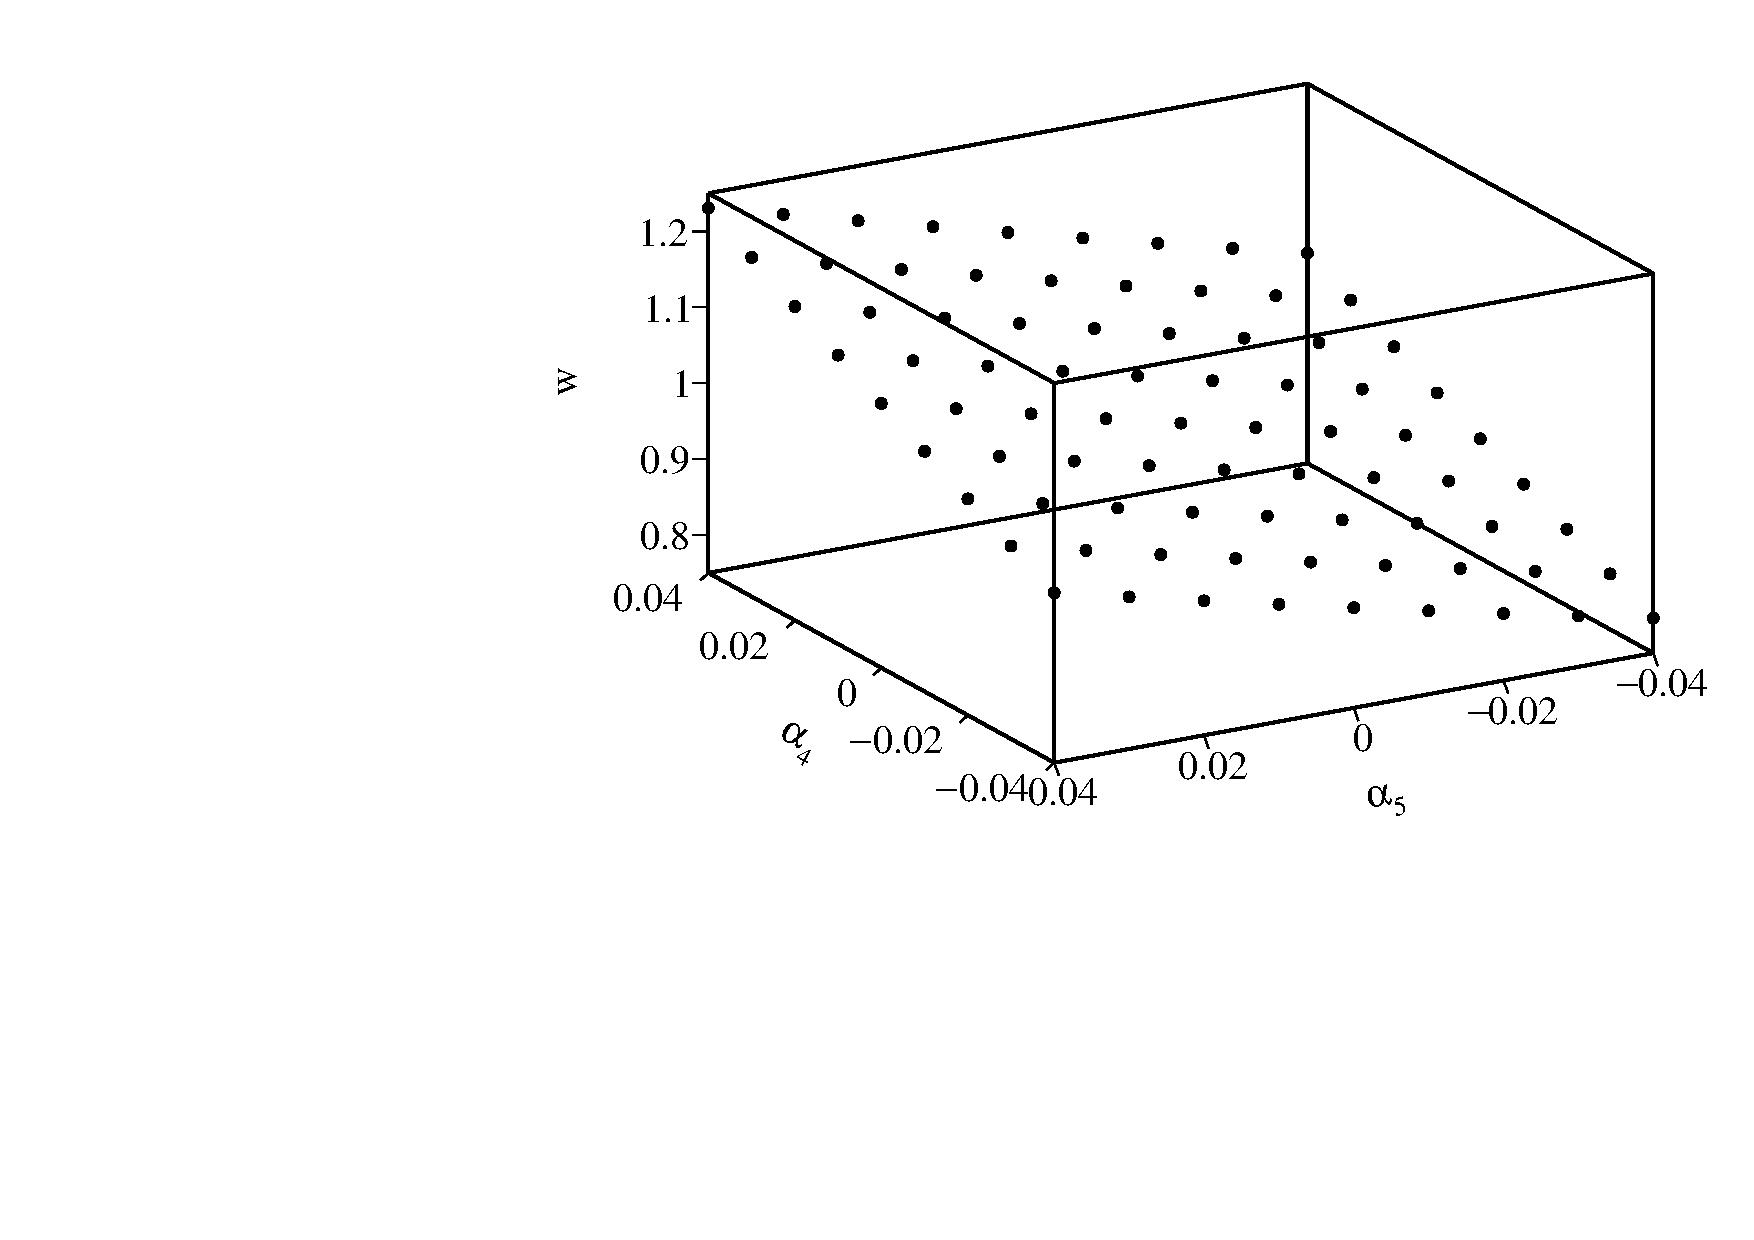
\includegraphics[width=0.5\textwidth]{PhysicsAnalysis/Plots/EventWeights/1400GeV/EventWeightsForEvent100001009_1400GeV_SPFOs_kt_0p70_10Bins_Start_0_End_10_1400GeV_Raw.pdf}}
\subfloat[]{\label{fig:weight2}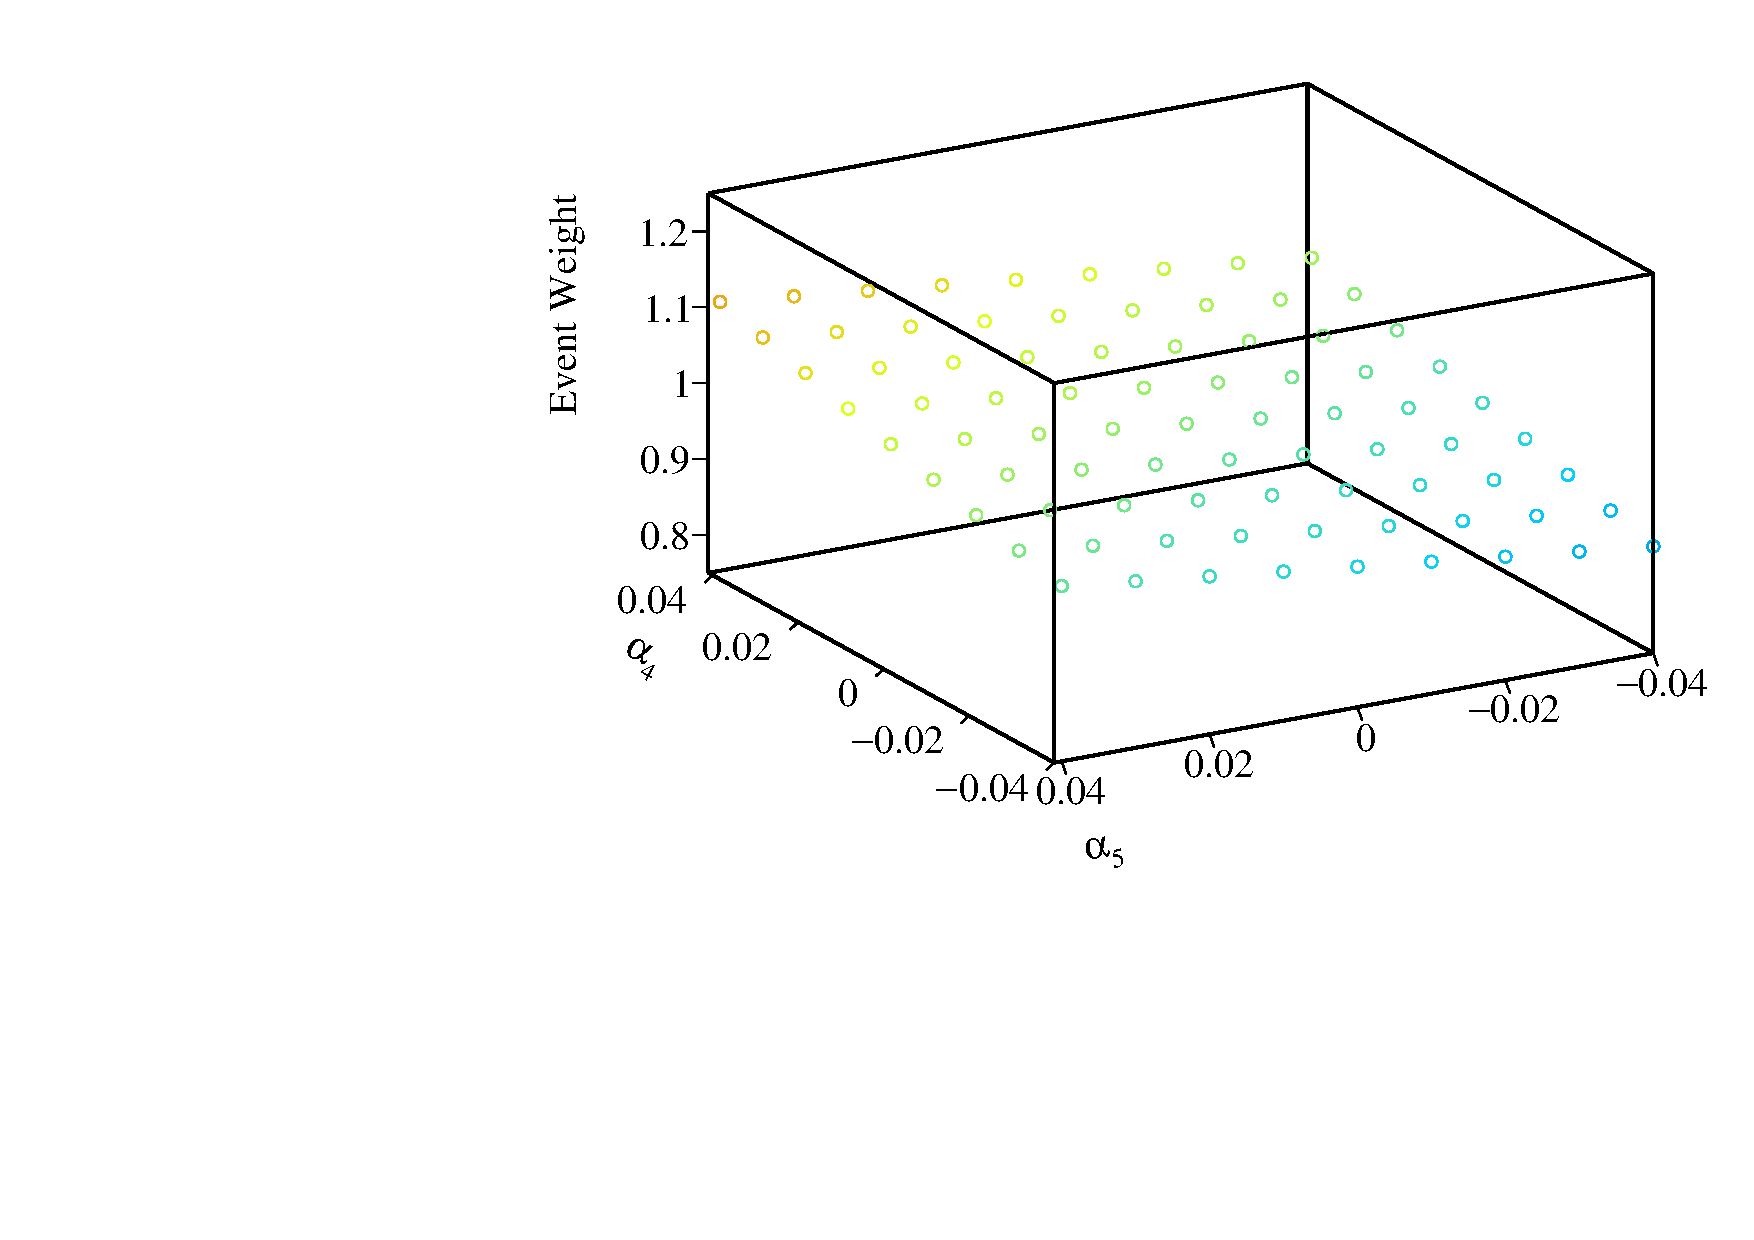
\includegraphics[width=0.5\textwidth]{PhysicsAnalysis/Plots/EventWeights/1400GeV/EventWeightsForEvent100001014_1400GeV_SPFOs_kt_0p70_10Bins_Start_0_End_10_1400GeV_Raw.pdf}} \hfill
\subfloat[]{\label{fig:weight3}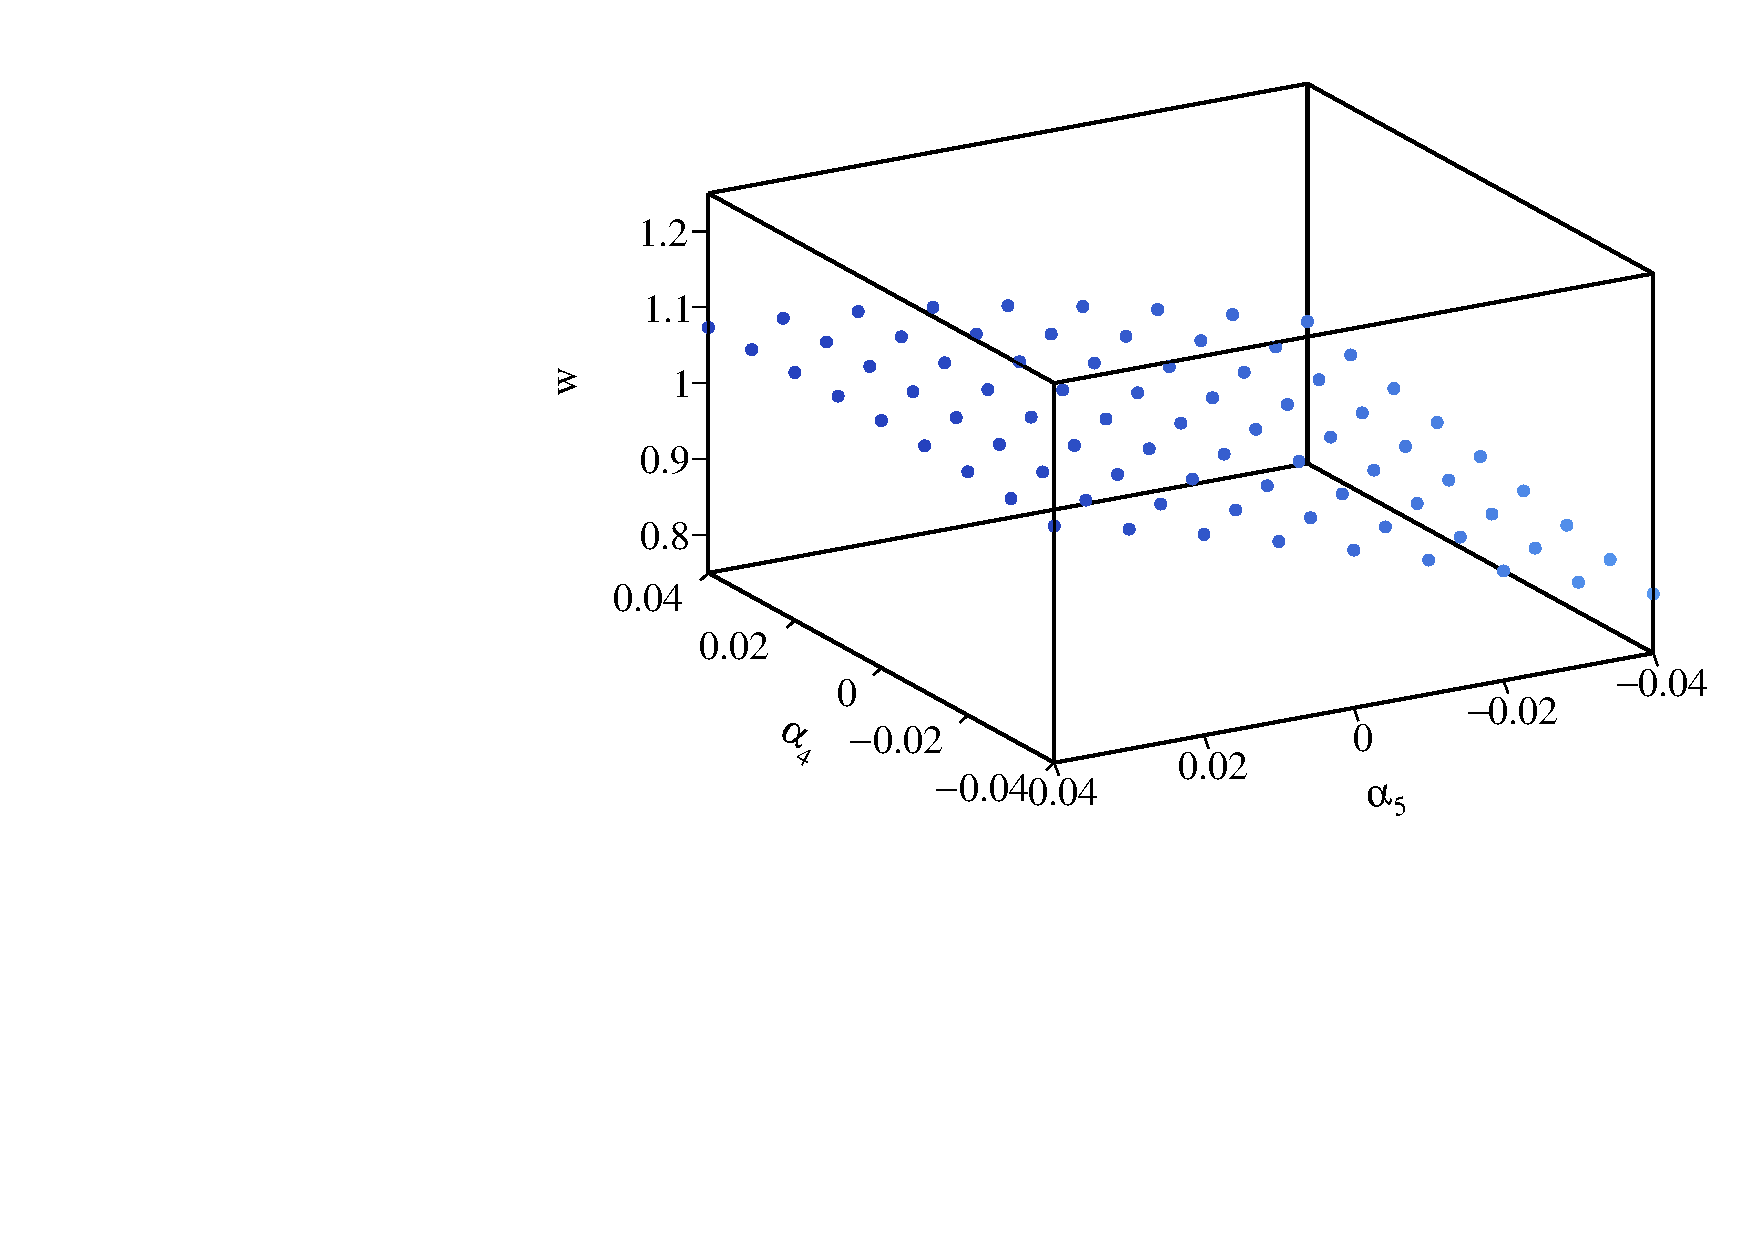
\includegraphics[width=0.5\textwidth]{PhysicsAnalysis/Plots/EventWeights/1400GeV/EventWeightsForEvent100001044_1400GeV_SPFOs_kt_0p70_10Bins_Start_0_End_10_1400GeV_Raw.pdf}}
\subfloat[]{\label{fig:weight4}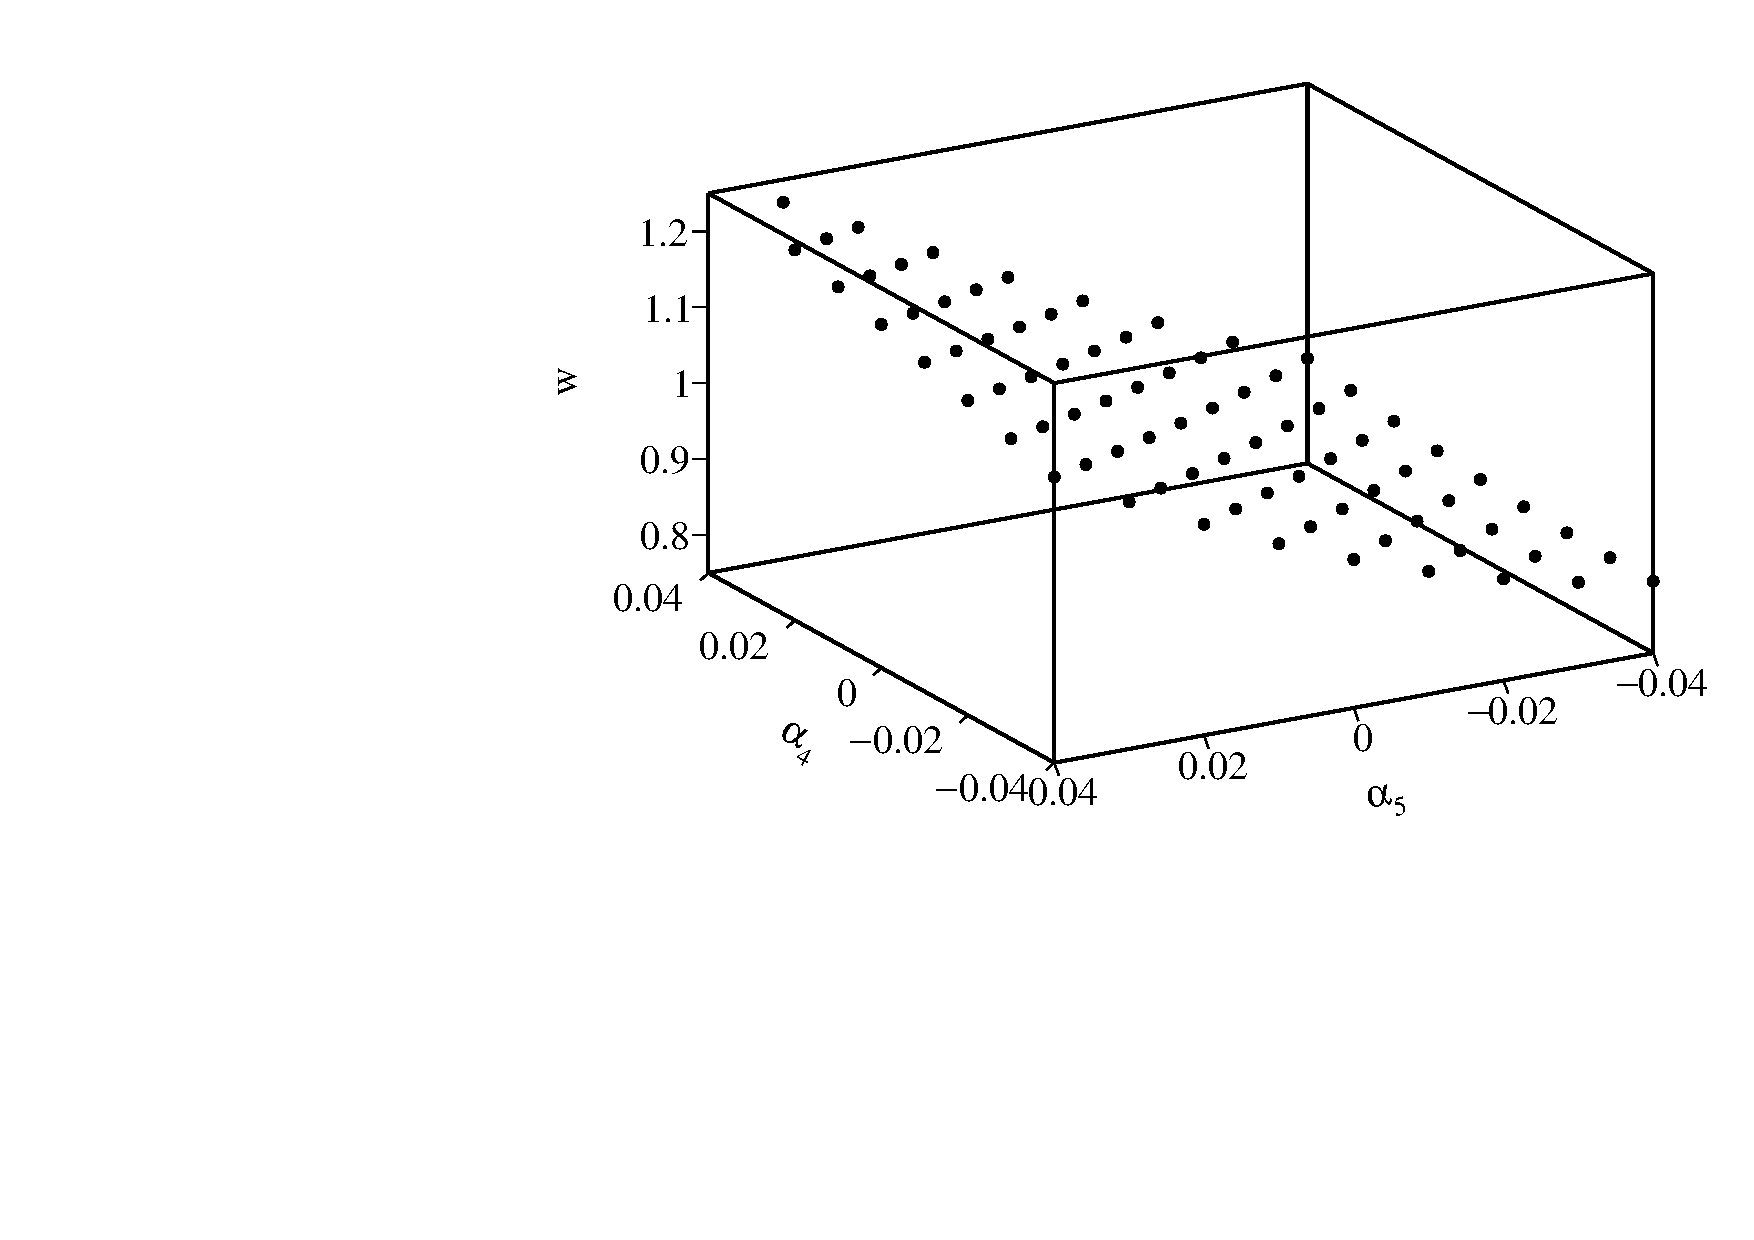
\includegraphics[width=0.5\textwidth]{PhysicsAnalysis/Plots/EventWeights/1400GeV/EventWeightsForEvent100001051_1400GeV_SPFOs_kt_0p70_10Bins_Start_0_End_10_1400GeV_Raw.pdf}}
\caption[Event weights from Whizard for 1.4TeV \nu{\nu}qqqq final state events.]{A selection of plots showing how the event weight changes when varying the anomalous couplings $\alpha_{4}$ and $\alpha_{5}$ for 1.4TeV \nu{\nu}qqqq final state events.}
\label{fig:eventweights1400raw}
\end{figure}

The cross check shows that the most sensitive channel to the anomalous gauge couplings is the \nu{\nu}qqqq indicating that the best sensitivity measurement should focus upon this channel, which is the aim of this analysis.

The CLIC experiment has a repository of simulated and reconstructed samples that can be used for physics analyses, however, for the relevant final states there is no way to calculate the event weights for these samples. Therefore, new samples for which reweighting is possible were created and processed through the CLIC reconstruction chain. New samples were created only for the \nu{\nu}qqqq final state as the l{\nu}qqqq and llqqqq final states have a significantly lower sensitivity. As will be shown in subsequent chapters, the application of an isolated lepton finder in the selection processor will largely veto the l{\nu}qqqq and llqqqq final states, therefore, the absence of weight information for these final states will not significantly affect the sensitivity measurement based on the \nu{\nu}qqqq final state.

\begin{table}[h!]
\centering
\begin{tabular}{ l l l l l}
\hline
Final State & Cross Section [fb] & Cross Section [fb] & Percentage & CLIC Cross Section \\ 
& ($\alpha_{4} = \alpha_{5} = 0.00$) & ($\alpha_{4} = \alpha_{5} = 0.05$) & Change[\%] & [fb] \\ 
\hline
$\text{e}^{+}\text{e}^{-} \rightarrow \nu{\nu}\text{qqqq}$ & 20.8 & 34.6 & +66.3 & 24.7 \\
$\text{e}^{+}\text{e}^{-} \rightarrow \text{l}{\nu}\text{qqqq}$ & 112 & 113 & +0.9 & 115.3 \\
$\text{e}^{+}\text{e}^{-} \rightarrow \text{llqqqq}$ & 59.7 & 68.6 & +14.9 & 62.1 \\
\hline
\end{tabular}
\caption{Cross section for selected processes for given value of $\alpha_{4}$ and $\alpha_{5}$ at 1.4 TeV.}
\label{table:crosssectionsensitivity1400}

\begin{tabular}{ l l l l l}
\hline
Final State & Cross Section [fb] & Cross Section [fb] & Percentage & CLIC Cross Section \\ 
& ($\alpha_{4} = \alpha_{5} = 0.000$) & ($\alpha_{4} = \alpha_{5} = 0.005$) & Change[\%] & [fb] \\ 
\hline
$\text{e}^{+}\text{e}^{-} \rightarrow \nu{\nu}\text{qqqq}$ & 51.2 & 77.7 & +51.8 & 71.5 \\
$\text{e}^{+}\text{e}^{-} \rightarrow \text{l}{\nu}\text{qqqq}$ & 111.9 & 115.9 & +3.6 & 106.6 \\
$\text{e}^{+}\text{e}^{-} \rightarrow \text{llqqqq}$ & 169.7 & 161.7 & -4.9 & 169.3 \\
\hline
\end{tabular}
\caption{Cross section for selected processes for given value of $\alpha_{4}$ and $\alpha_{5}$ at 3 TeV.}
\label{table:crosssectionsensitivity3000}
\end{table}

\section{Validation of New Samples}

An identical setup to that used for the official CLIC sample was used for the event generation and reconstruction. Several reconstructed level distributions were compared to the official CLIC samples and all were found to be comparably to each other. A selection of these distributions is shown in figure \ref{fig:cliccomp}.

\begin{figure}
\centering
\subfloat[Visible Mass]{\label{fig:cliccomp1}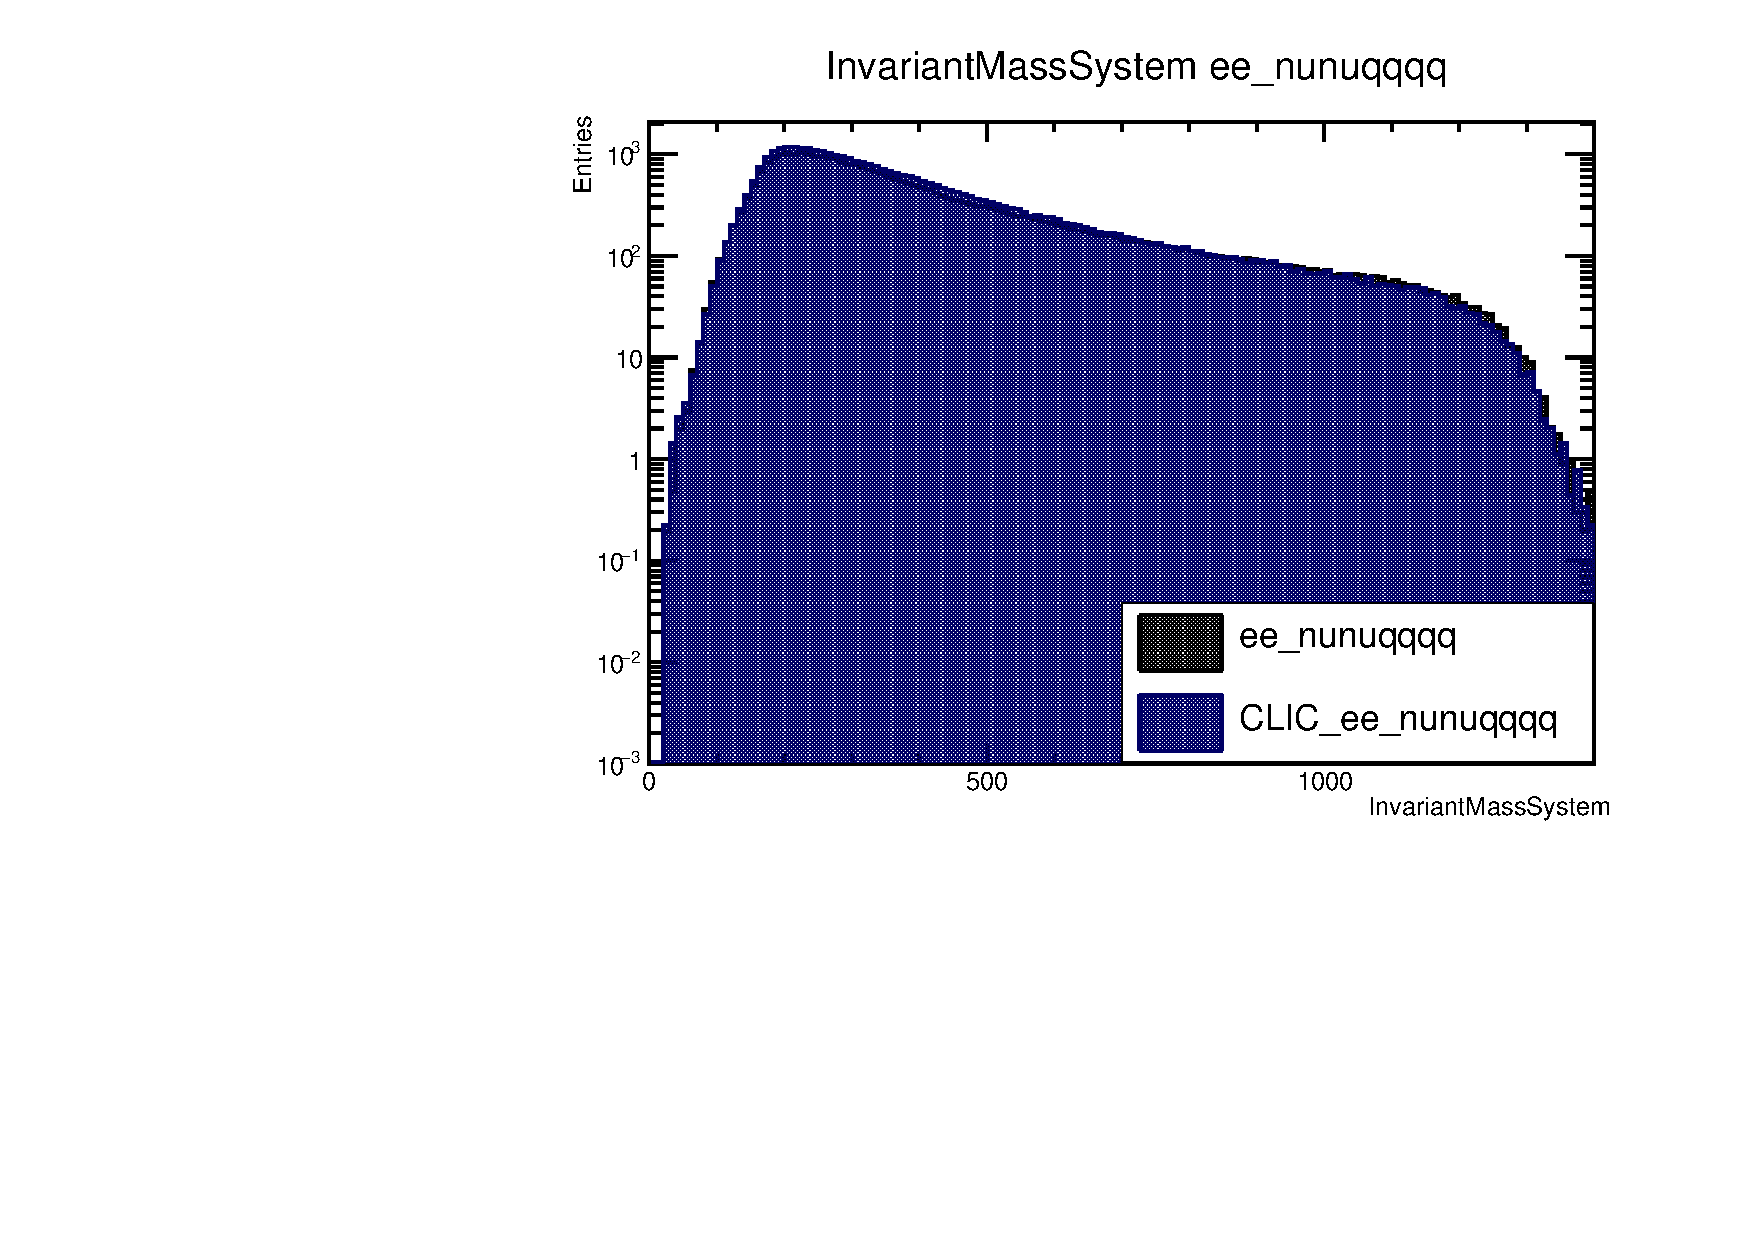
\includegraphics[width=0.5\textwidth]{PhysicsAnalysis/Plots/CLICSampleComparison/InvariantMassSystem.pdf}}
\subfloat[$\text{cos}\theta_{Missing}$ - The cosine of the polar angle of the missing momentum for an event.]{\label{fig:cliccomp2}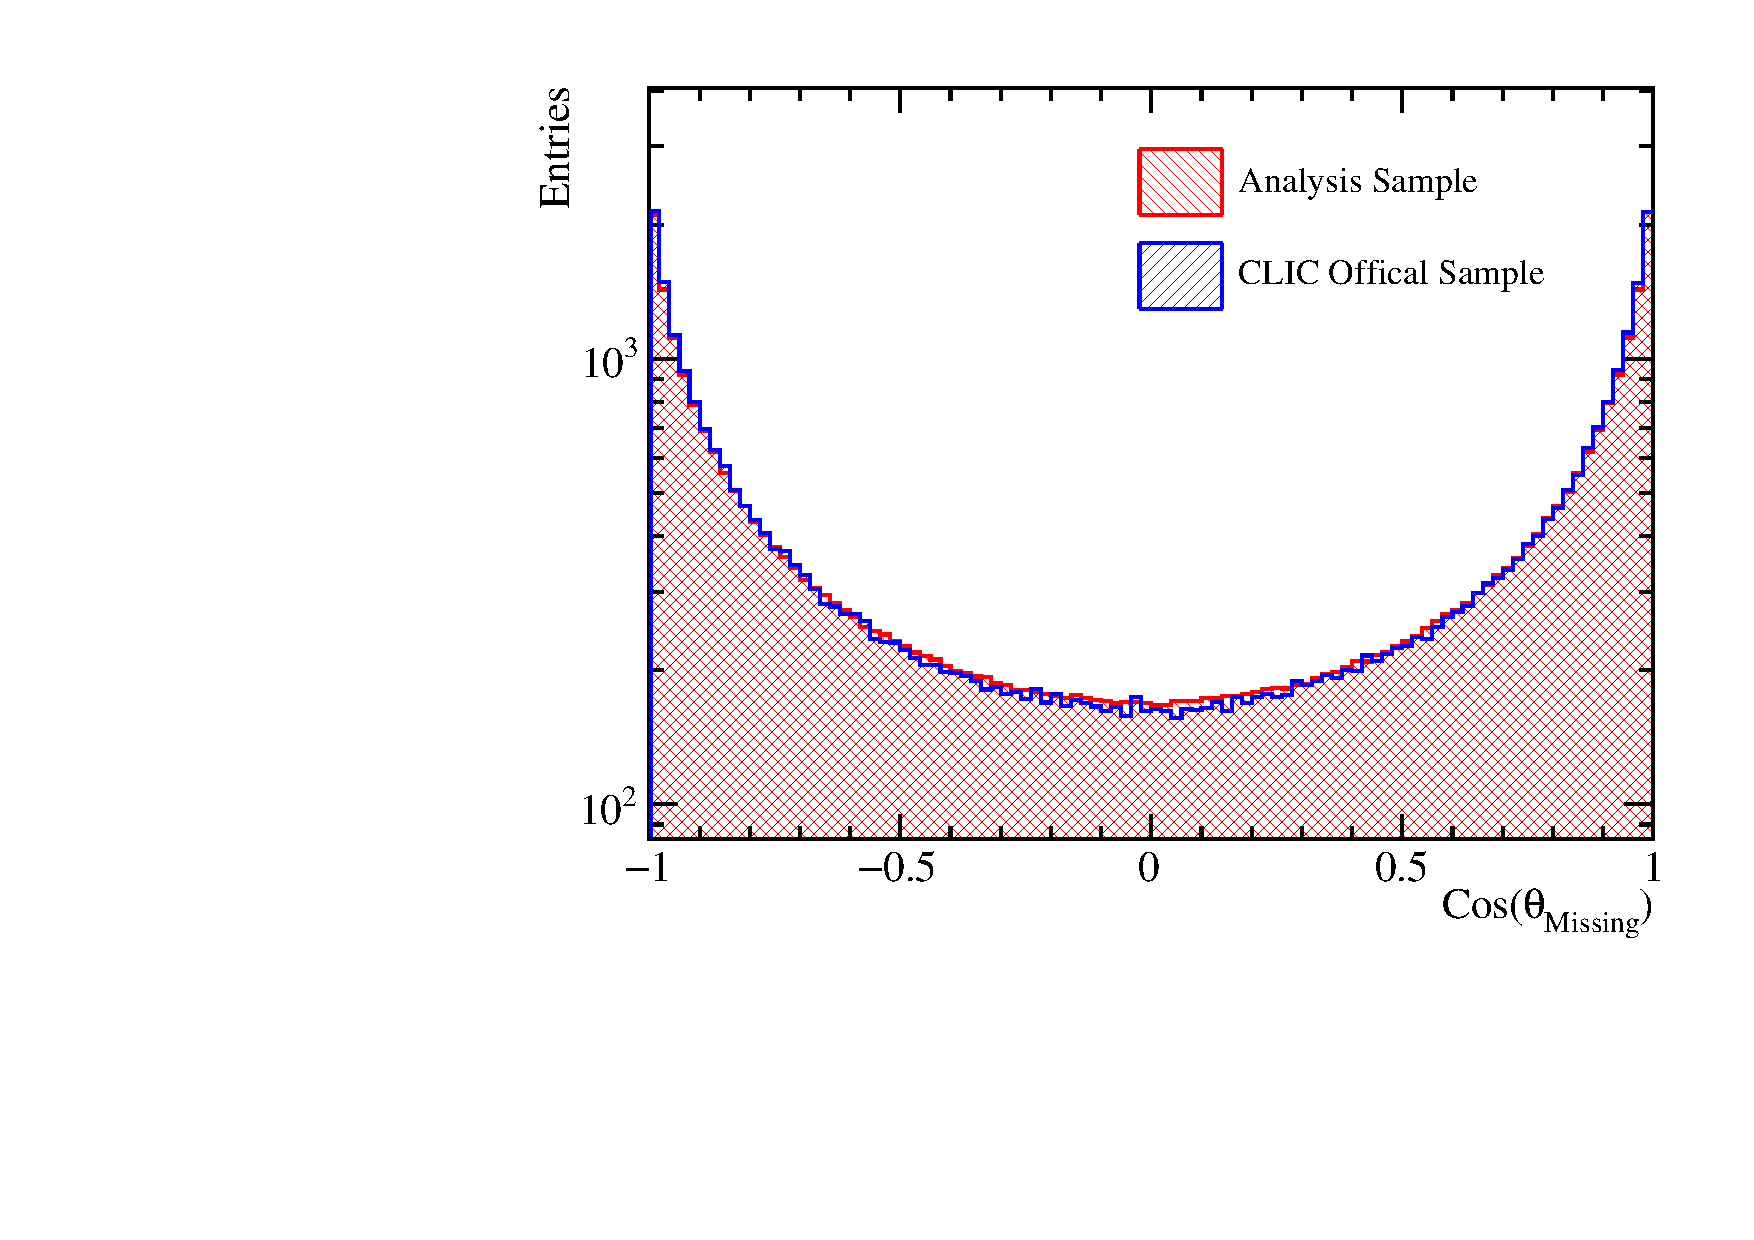
\includegraphics[width=0.5\textwidth]{PhysicsAnalysis/Plots/CLICSampleComparison/CosThetaMissing.pdf}} 
\caption[Comparison of various distributions between samples used in this analysis and the official CLIC samples for the \nu{\nu}qqqq final state.]{Comparison of various distributions between samples used in this analysis and the official CLIC samples for the \nu{\nu}qqqq final state.}
\label{fig:cliccomp}
\end{figure}

\section{Simulation and Reconstruction}

The CLID\_ILD detector \cite{arXiv:1006.3396} was simulated using the GEANT4 wrapper MOKKA and events were reconstructed using the MARLIN framework. Using the CLIC\_ILD detector for this analysis provides access to the background samples created by the CLIC collaboration. The CLIC\_ILD detector has a 60 layer scintillator-tugsten HCal in comparison to the 48 layer HCal found in the default ILD detector. The increase in thickness of the detector for the CLIC experiment is needed to compensate for the effects of leakage at the higher energies that will be seen by the CLIC experiment in comparison to the ILC. Practically speaking the ILD and CLIC\_ILD detectors are otherwise identical.

Version of MOKKA used is 08-00-03. MarlinPandora version used is v00-09-02. PandoraPFANew version v00-09 \cite{arXiv:0907.3577, arXiv:1209.4039}.

\section{Analysis Processor and Jet Pairing} \label{sec:jetpairing}

For both signal and background events the FastJet processor is run to cluster the events into 4 jets. These are then assumed to be from the decays of the vector boson scattering bosons and the jets are paired up on the assumption that the correct pair arises when the invariant masses of the two pairs are closest together. The longitudinally invariant kt jet algorithm in exclusive modes is used for the jet clustering.
This jet algorithm proceeds as follows:

\begin{itemize}
\item For each pair of particles i and j work out the kt distance and beam distance $d_{iB} = p_{t}^{2}$.
\begin{equation}
d_{ij} = \text{min}(p_{ti}^{2}, p_{tj}^{2}){\Delta}R^{2}_{ij}/R^{2}
\end{equation}
where ${\Delta}R^{2}_{ij} = (y_{i} - y_{j})^2 + (\phi_{i} - \phi_{j})^2$.  $p_{t}$ is the transverse momentum of the particle with respect to the beam axis, $y_{i}$ is the rapidity of particle i and $\phi_{i}$ is the azimuthal angle of particle i. $R$ is a configurable parameter that typically is of the order of 1.
\item Find the minimum distance $d\text{min}$ of all the $k_{t}$ and beam distances. If the minima occurs for a $k_{t}$ distance, merge particles i and j, summing their 4-momenta in the energy combination scheme (also configurable). If the beam distance is the minimum declare particle i to be apart of the "beam" jet and remove it from the list of particles and not included in the final output jets.
\item Repeat until no particles are left or the requested number of jets have been created (or optionally apply a minimum $d_{cut}$ where clustering stops, but here the event is forced into 4 jets).
\end{itemize}

An inclusive mode is available, but not applied here as the finally number of jets in the output varies and events need to be clustered into 4 jets in this analysis.  Two other clustering modes were considered, but were found to be inappropriate for this analysis as is shown in figure \ref{fig:eventweights1400raw}. They were:

\begin{itemize}
\item The kt algorithm for e+e  colliders (or Durham algorithm) where $d_{ij} = 2\text{min}(E_{i}^{2}, E_{j}^{2})(1-cos\theta_{ij})$ and $d_{iB}$ is not used. $\theta_{ij}$ is the opening angle of the particles. In the collinear limit this corresponds to the relative transverse momentum of the particles. Unlike the other algorithm choices this is not invariant to boosts along the beam direction as in theory for e+e  colliders the collision should occur with no net 3 momentum, unlike hadron colliders where the events have a net 3-momentum. However, the presence of ISR and beam effects makes this algorithm inappropriate for CLIC. The major failure of this algorithm choice is the absence of diB as this associates too many background particles to jets when applied at CLIC.
\item The Cambridge/Aachen jet algorithm where $d_{ij} = {\Delta}R_{ij}^{2}/R^2$ and $d_{iB} = 1$. This algorithm gave poor performance as it is based entirely on spacial information and does not account for the transverse momentum or energy of the particles being grouped. In essence this is a cone clustering algorithm with a cone radius defined through ${\Delta}R_{ij} = R$, which even for large R was found to throw away too much energy in the event to be useful for this analysis. This algorithm can be useful for events with small jets that are highly boosted, but in this case the jets are too large to be successfully merged.
\end{itemize}

\begin{figure}
\centering
\subfloat[]{\label{fig:invariantmassalgoveto1400GeV}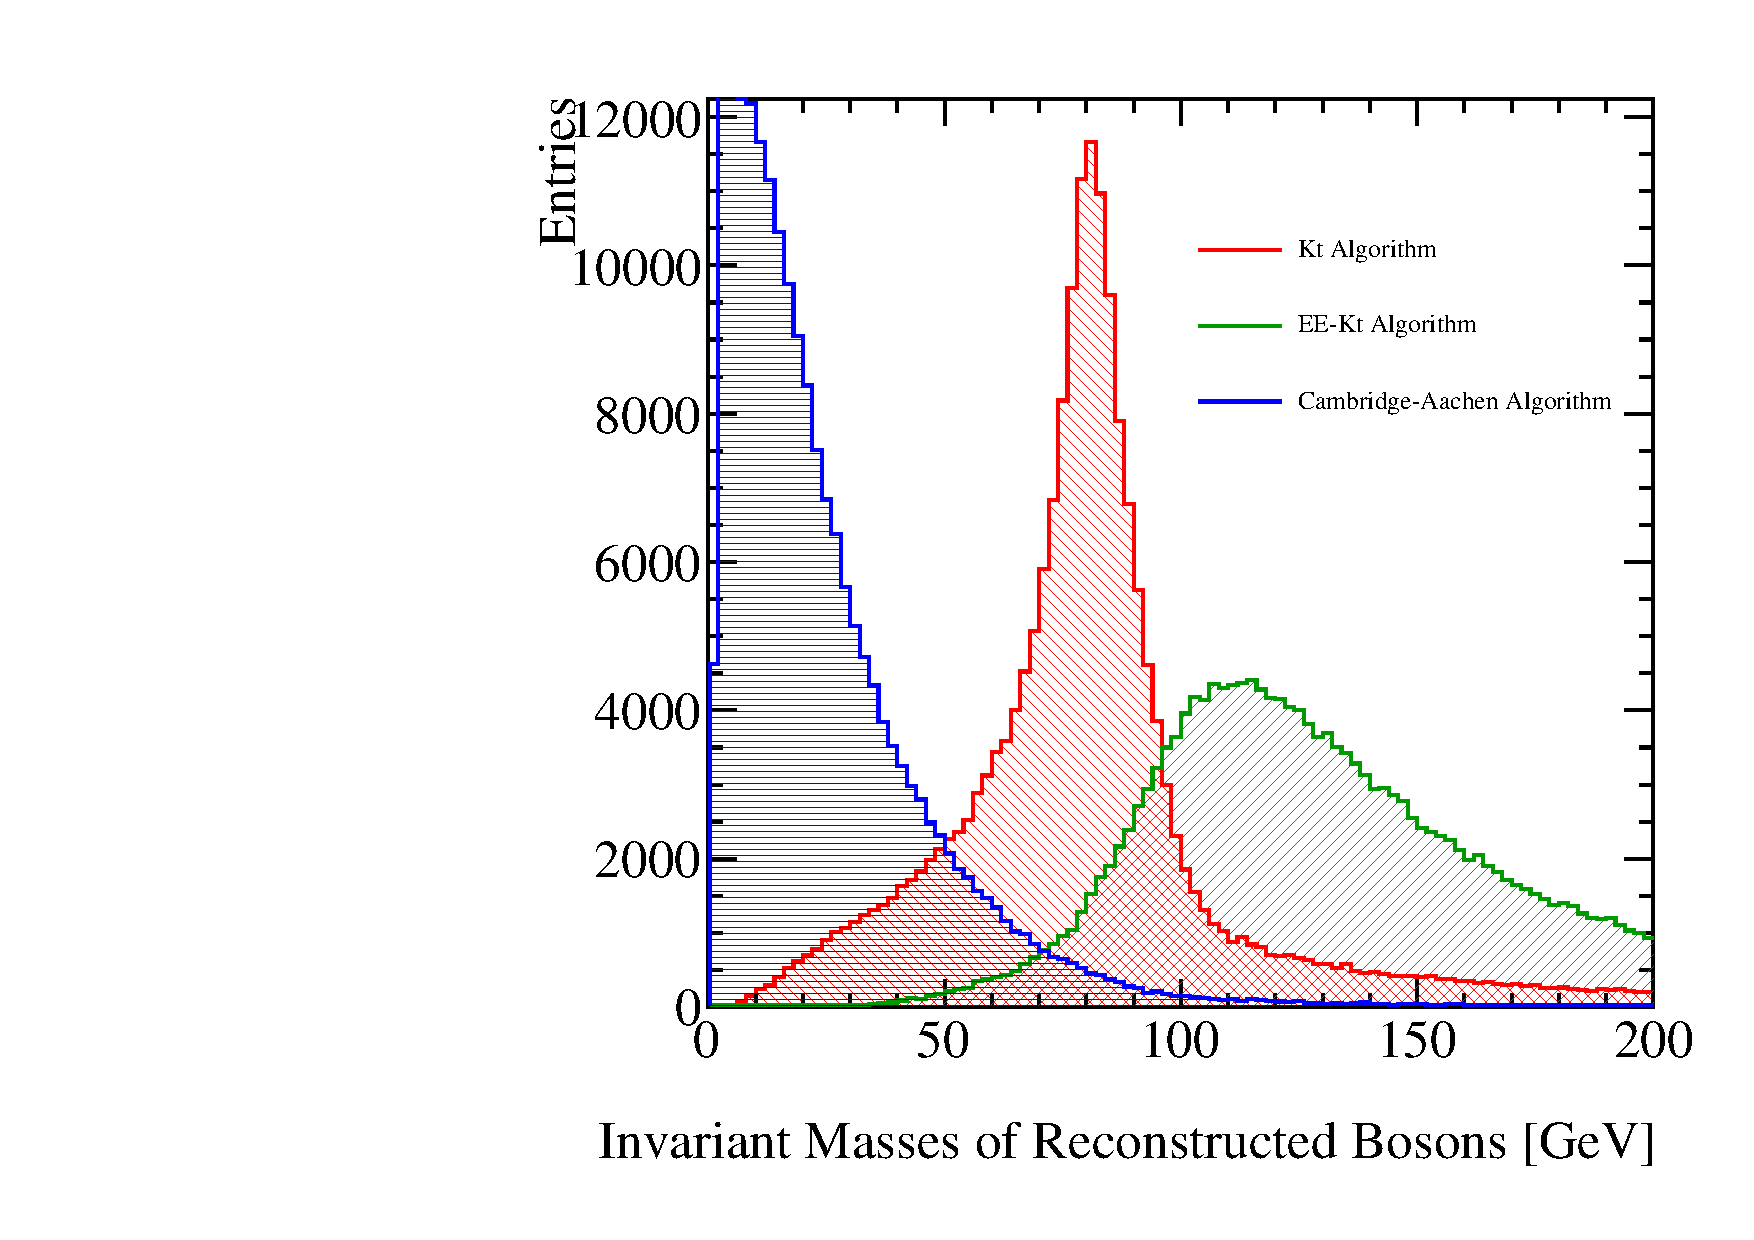
\includegraphics[width=0.5\textwidth]{PhysicsAnalysis/Plots/SimpleInvMassPlot/InvariantMassesAlgorithmVeto.pdf}}
\subfloat[]{\label{fig:invariantmassalgoveto3000GeV}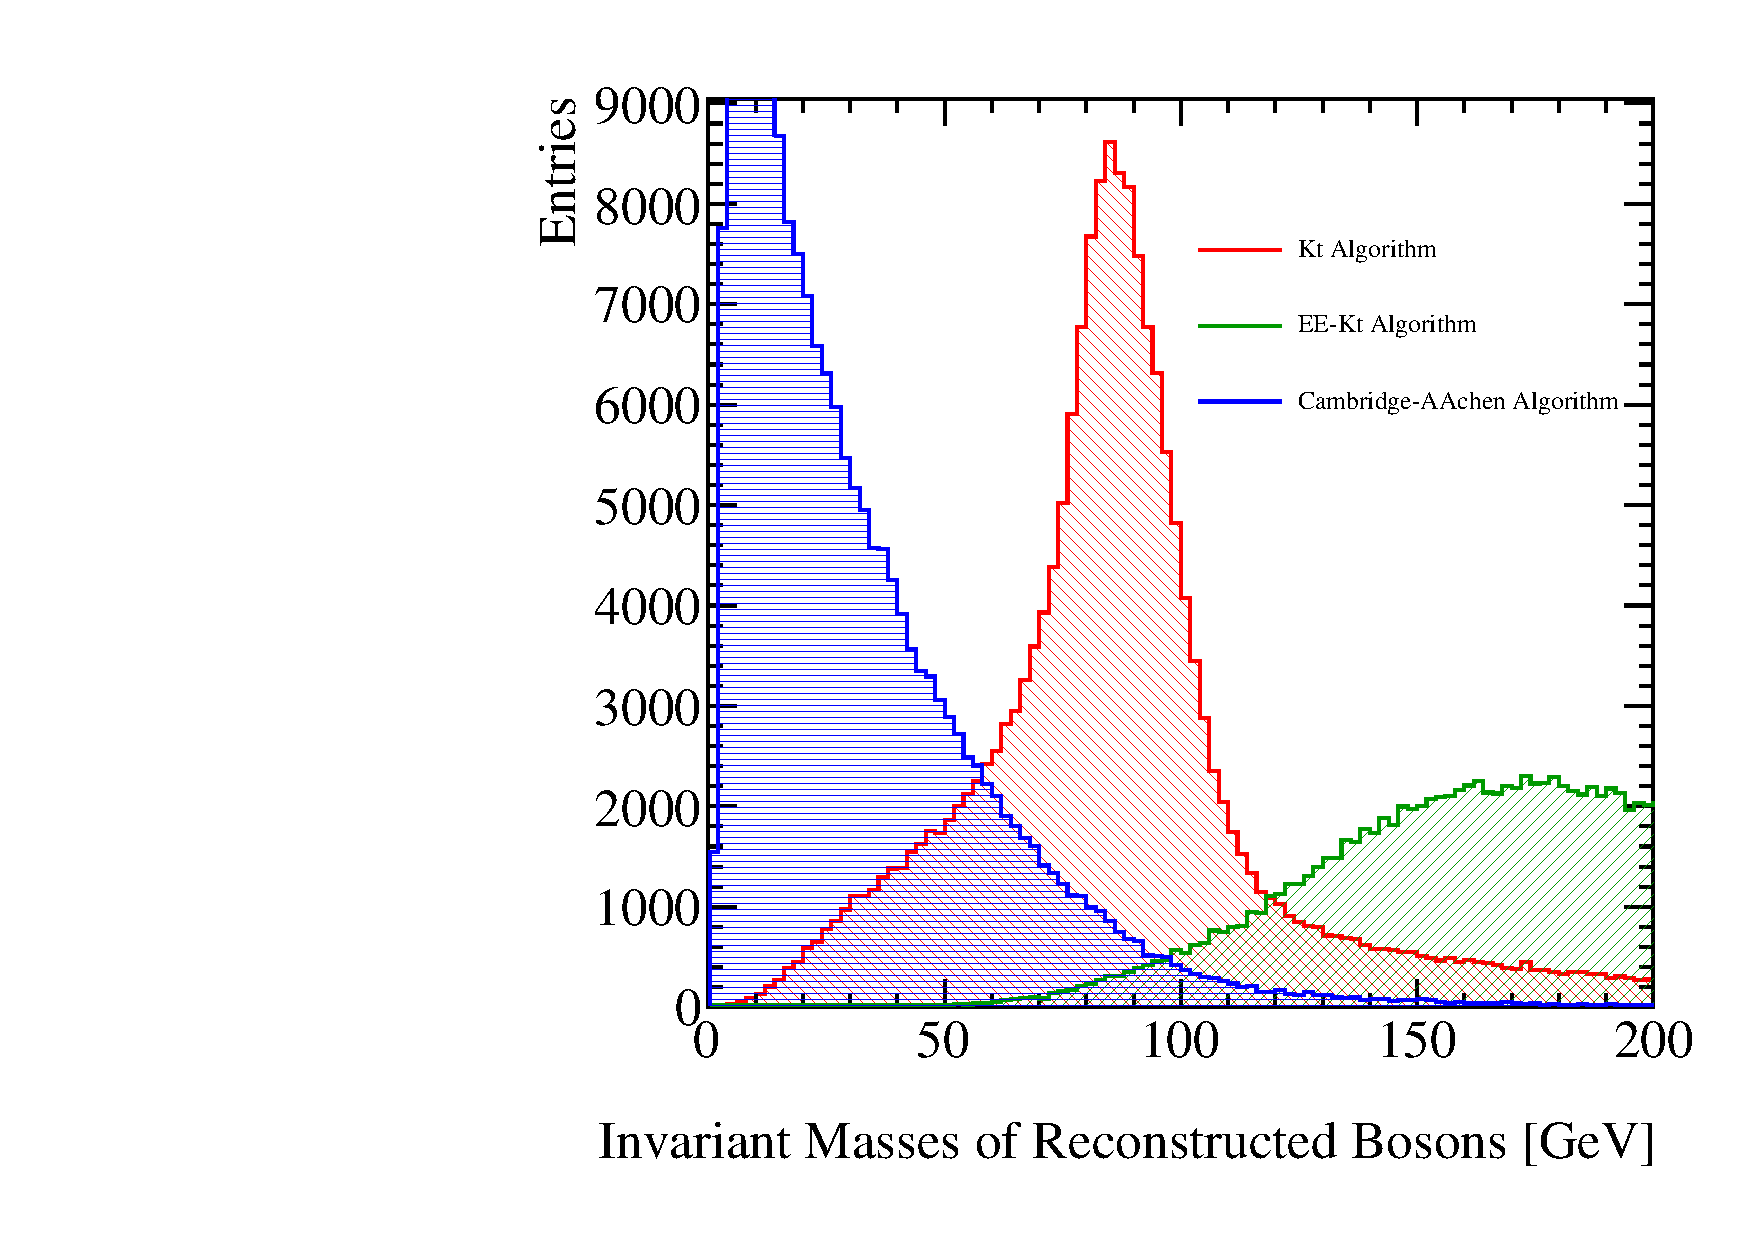
\includegraphics[width=0.5\textwidth]{PhysicsAnalysis/Plots/SimpleInvMassPlot/InvariantMassesAlgorithmVeto3000GeV.pdf}}
\caption[Reconstructed invariant masses for different choices of jet algorithm for 1.4 TeV and 3 TeV \nu{\nu}qqqq events.]{Reconstructed masses for different choices of jet algorithm for 1.4 TeV and 3 TeV \nu{\nu}qqqq events. These masses arise by forcing the reconstructed events into 4 jets and then pairing up the jets into pairs such that the reconstructed invariant masses of the pairs are closest to each other. These samples should be dominated by vector boson scattering involving pairs of W bosons and so it is expected that a peak at the W boson true mass should be observed. As this does not occur for the Cambridge-Aachen algorithm or the ee\_kt algorithm they were deemed unsuitable for this analysis at both 1.4 and 3 TeV. In the case of the kt algorithm and the ee\_kt algorithm an R parameter of 0.7 was used.}
\label{fig:eventweights1400raw}
\end{figure}

Alongside the jet clustering an isolated lepton finder is run to help reject back- ground events containing high energy leptons. The LCFIPlus vertex processor is also run on these events once clustered into jets to produce a value for the B and C tag likelihood. This information is also used for background rejection instead of contributing to the sensitivity of the event to the anomalous couplings. The LCFIPlus vertex tagger was trained using events of $\text{e}^{+}\text{e}^{-}\rightarrow \text{Z}\nu\nu \rightarrow \text{q}\bar{\text{q}}\nu\nu$ for q = u,d,s,c,b.

Finally, an analysis processor is run, which calculates a number of variables used downstream in the analysis. Included in these are:
\begin{itemize}
\item Number of PFOs in the jets and the paired up bosons.
\item Number of charged PFOs in the jets and paired up bosons.
\item Highest energy PFO: energy, momentum, transverse momentum, $cos\theta$.
\item Highest energy electron PFO: energy, momentum, transverse momentum, $cos\theta$.
\item Highest energy muon PFO: energy, momentum, transverse momentum, $cos\theta$.
\item Highest energy photon PFO: energy, momentum, transverse momentum, $cos\theta$.
\item (If in existence) Highest and second highest energy isolated lepton: energy, momentum, transverse momentum, $cos\theta$.
\item Bosons: energy, momentum, transverse momentum, $cos\theta$.
\item Invariant mass of the boson pair.
\item Jets: energy, momentum, transverse momentum, $cos\theta$.
\item $Cos\theta$ Of the missing 3-momentum vector.
\item Recoil mass.
\item Invariant mass of the visible system.
\item $y_{i}$, $y_{i+1}$. Jet clustering parameters ranging from i = 0 to 6.
\item $Cos\theta^{*}_{Jet}$.  This is the opening angle of a pair of jets, assumed to be from a signle boson, in the rest frame of the boson.
\item $Cos\theta^{*}_{Boson}$.  This is the opening angle of a pair of bosons, assumed to be from vector boson scattering, in the rest frame of the di-boson pair.
\item Transverse momentum and energy of the event.
\item Acolinearity of the jet pairs forming the bosons and the acoilinearity of the boson pair.
\item Principle thrust $T$ and the thrust axes $\bar{\textbf{n}}$. Note $\bar{\textbf{n}}$ is a unit vector. These are defined by the following equation
\begin{equation}
T = \text{max}_{\bar{\textbf{n}}} (\frac{\Sigma_{i} \textbf{p}_{i}.\bar{\textbf{n}}}{\Sigma_{i} |\textbf{p}_{i}|^{2}})
\end{equation}
\item The major and minor thrust values. These are defined with respect to the thrust axes $\bar{\textbf{n}}$ in the following way:
\begin{equation}
T = \text{max}_{\bar{\textbf{n}}_{major}} (\frac{\Sigma_{i} \textbf{p}_{i}.\bar{\textbf{n}}_{major}}{\Sigma_{i} |\textbf{p}_{i}|^{2}})
\end{equation}
where $\bar{\textbf{n}}_{major}.\bar{\textbf{n}} = \textbf{0}$. Similarly the minor thrust value is defined as 
\begin{equation}
T = \frac{\Sigma_{i} \textbf{p}_{i}.\bar{\textbf{n}}_{minor}}{\Sigma_{i} |\textbf{p}_{i}|^{2}}
\end{equation}
where $\bar{\textbf{n}}_{minor}.\bar{\textbf{n}} = \bar{\textbf{n}}_{minor}.\bar{\textbf{n}}_{major} =\textbf{0}$
\item Sphericity. This is defined using the sphericity tensor $S^{ab}$ defined as:
\begin{equation}
S^{ab} = \frac{\Sigma_{i}p^{\alpha}_{i}p^{\alpha}_{j}}{\Sigma_{i,\alpha=1,2,3}|p^{\alpha}_{i|^{2}}}
\end{equation}
Where $p_{i}$ are the components of the momenta of particle i in the frame of the detector and the sum runs over all particles in the event. Sphericity is defined as $\text{S} = \frac{3}{2}(\lambda_{2} + \lambda_{3})$, where $\lambda_{i}$ are the eigenvalues of the sphericity tensor defined such $\lambda_{1} \geq \lambda_{2} \geq \lambda_{3}$.  This provides a measure of how spherical the reconstructed event topology is with isotropic events having $S \approx 1$, while two jet events have $S \approx 0$.  (Also $\lambda_{1} + \lambda_{2} + \lambda_{3} = 1$.)
\item Aplanarity. Aplanarity is defined as $\frac{3}{2} \lambda_{3}$ where $\lambda_{3}$ is an eigenvalue of the sphericity tensor.  This provides a measure of whether an event is linear or planar.
\item B and C tag values for the jets, the min and max B and C tag values for the bosons.
\end{itemize}

Alongside these variables, for the \nu{\nu}qqqq final state a number of Monte-Carlo variables are calculated for informative purposes and are not used in the analysis. These include:
\begin{itemize}
\item The quark and neutrino 4 momenta.
\item Invariant mass of boson pair using MC pairing and MC energy.
\item Invariant mass of boson pair using MC pairing and reconstructed jet energy.
\end{itemize}

\section{Methodology for Fitting}
It is necessary to discuss the fitting procedure in this analysis as the optimisation of the jet algorithms relies on this methodology. In this section only the signal events are considered to determine the underlying sensitivity of the CLIC detector to the anomalous couplings. This decision was made to save analysis of the large number of background samples in the optimisation of the jet reconstruction algorithms, while still optimising the algorithm on the physics of interest.

The sensitivity of CLIC to the anomalous gauge couplings is determined through the use of a $\chi^{2}$ fit to the distribution of $\text{cos}\theta^{*}_{Jets}$ where $\theta^{*}_{Jets}$ is the angle between the two jets produced from the hadronic decay of the W/Z boson in the rest frame of that boson.  The distribution of $\text{cos}\theta^{*}_{Jets}$ proved to be sensitive to the anomalous gauge couplings as shown in figure \ref{fig:costhetastarjets}.

Another distribution considered for the sensitivity study was  $\text{cos}\theta^{*}_{Bosons}$ where $\theta^{*}_{Bosons}$ is the angle between the two bosons produced in vector boson scattering in the rest frame of the boson pair.  This distribution was found to be less sensitive to the anomalous gauge couplings than $\text{cos}\theta^{*}_{Jets}$, which can be seen when comparing figures \ref{fig:costhetastarjets} and \ref{fig:costhetastarbosons}, and so was not considered for the rest of this study.  Furthermore, it was found that a two dimensional $\chi^{2}$ fit produced by combining $\text{cos}\theta^{*}_{Jets}$ and $\text{cos}\theta^{*}_{Bosons}$ did not improve the sensitivity significantly in comparison to $\text{cos}\theta^{*}_{Jets}$.

The $\text{cos}\theta^{*}_{Jets}$ variable was binned in histograms of 10 bins before begin converted into a value of $\chi^{2}$.  This binning was selected to maximise the number of bins in the distribution, while minimising the effect of large bin by bin fluctuations arising from individual events with large event weights.

\begin{figure}
\subfloat[1.4 TeV Events]{\label{fig:costhetastarjets1400GeV} 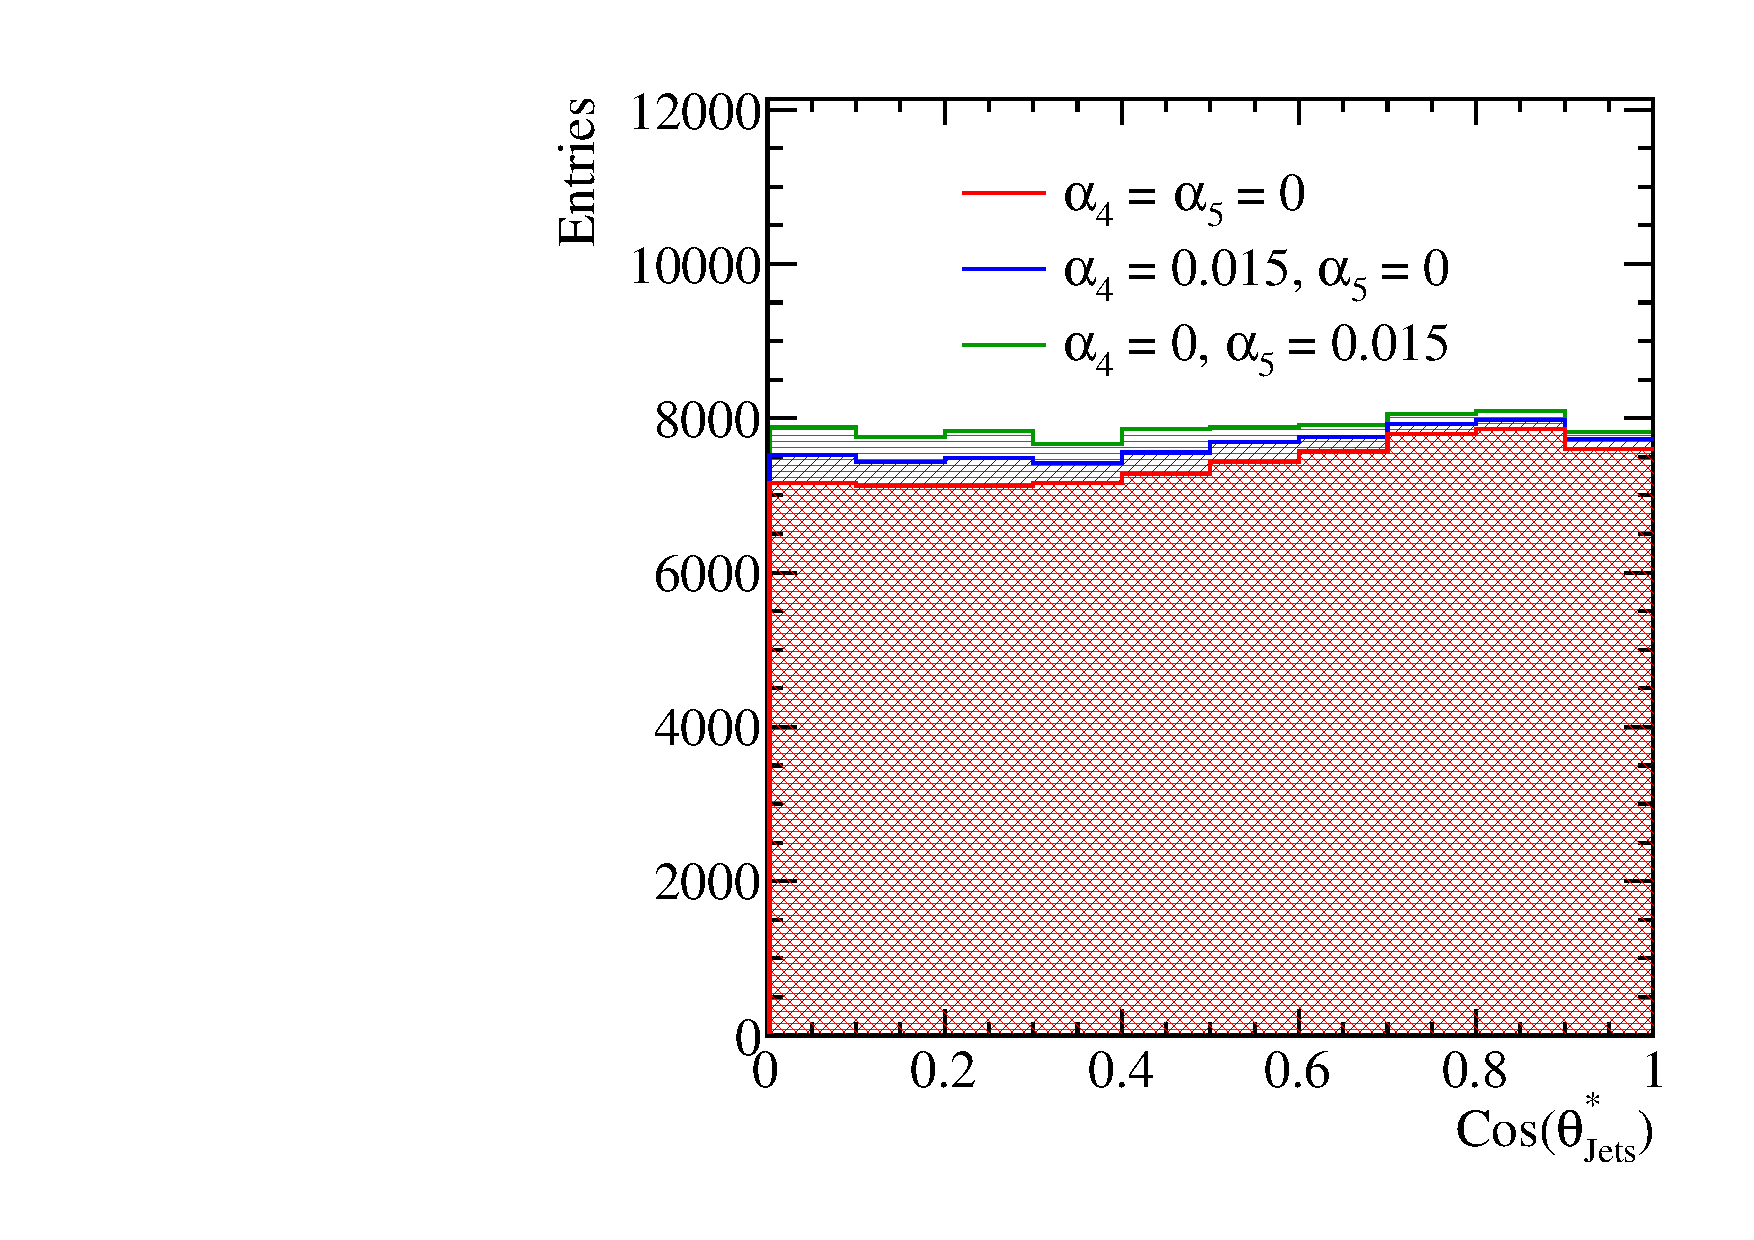
\includegraphics[width=0.5\textwidth]{PhysicsAnalysis/Plots/SensitiveDistributions/CosThetaStarSynJets_SPFOs_kt_0p70_1400GeV.pdf}}
\subfloat[3 TeV Events]{\label{fig:costhetastarjets3000GeV} 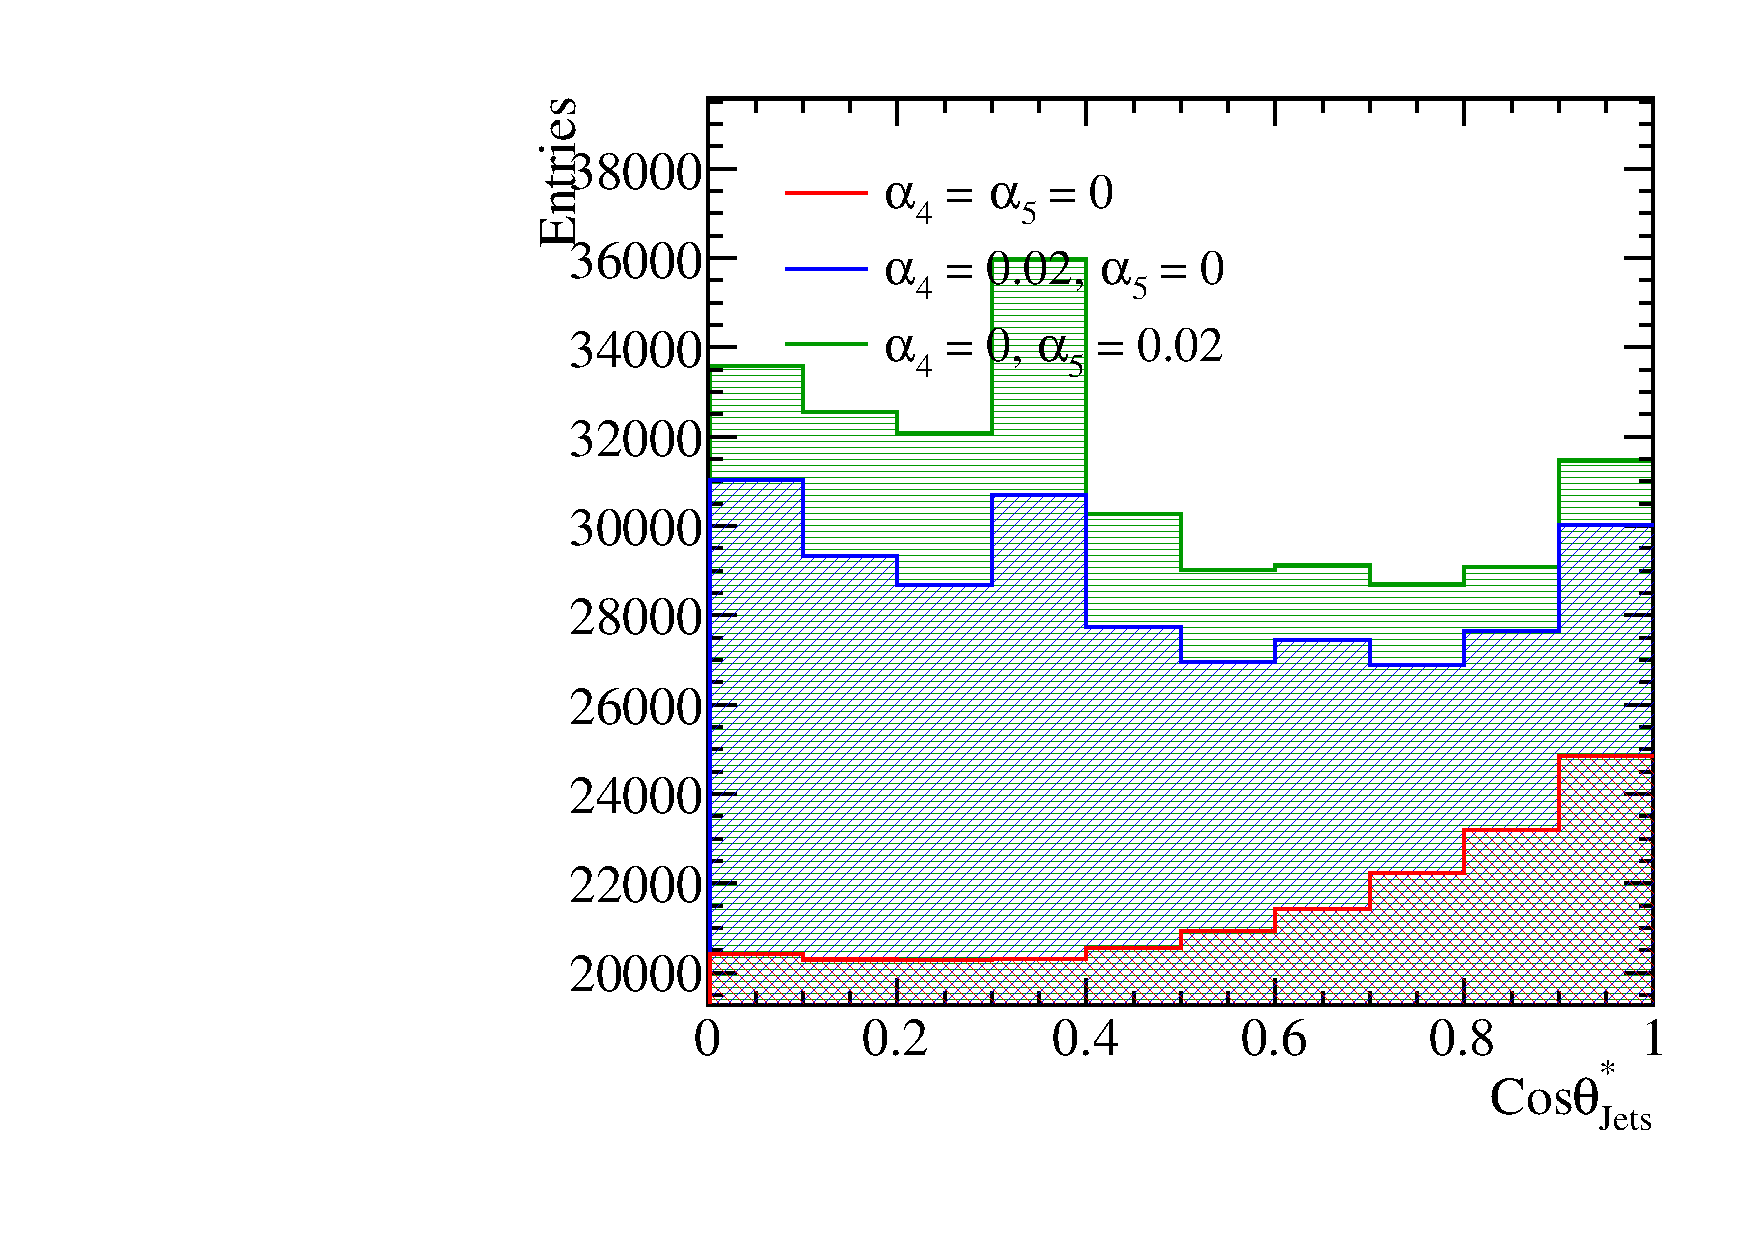
\includegraphics[width=0.5\textwidth]{PhysicsAnalysis/Plots/SensitiveDistributions/CosThetaStarSynJets_SPFOs_kt_0p70_3000GeV.pdf}}
\caption[Sensitivity of $\text{cos}\theta^{8}_{Jets}$ to the anomalous gauge couplings $\alpha_{4}$ and $\alpha_{5}$ at 1.4 and 3 TeV.]{Sensitivity of $\text{cos}\theta^{*}_{Jets}$ to anomalous couplings at 1.4 and 3 TeV. The jet algorithm used for this example was the longitudinally invariant kt algorithm with an R parameter of 0.7. This sample corresponds to pure signal of hadronic decays in vector boson scattering i.e. \nu{\nu}qqqq.}
\label{fig:costhetastarjets}
\end{figure}

\begin{figure}
\subfloat[1.4 TeV Events]{\label{fig:costhetastarbosons1400GeV} 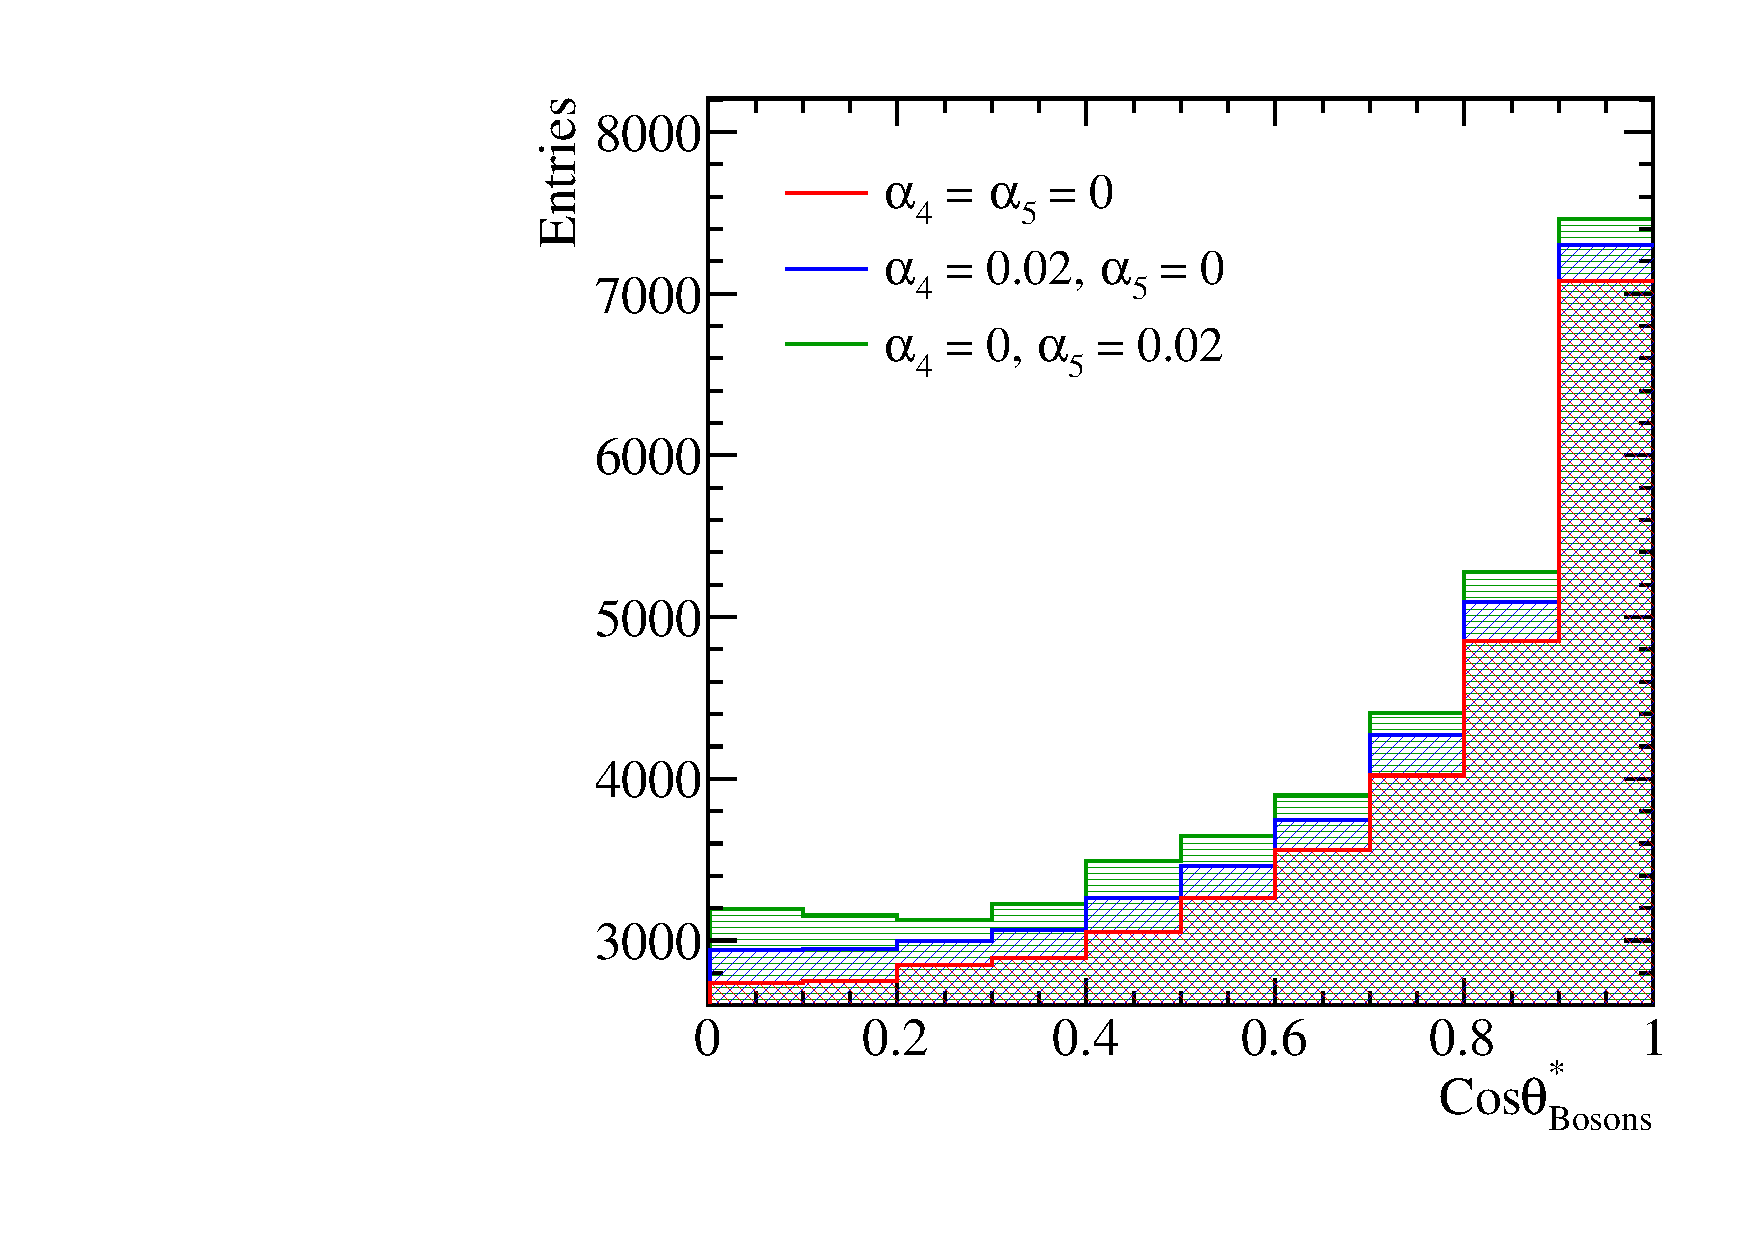
\includegraphics[width=0.5\textwidth]{PhysicsAnalysis/Plots/SensitiveDistributions/CosThetaStarSynBosons_SPFOs_kt_0p70_1400GeV.pdf}}
\subfloat[3 TeV Events]{\label{fig:costhetastarbosons3000GeV} 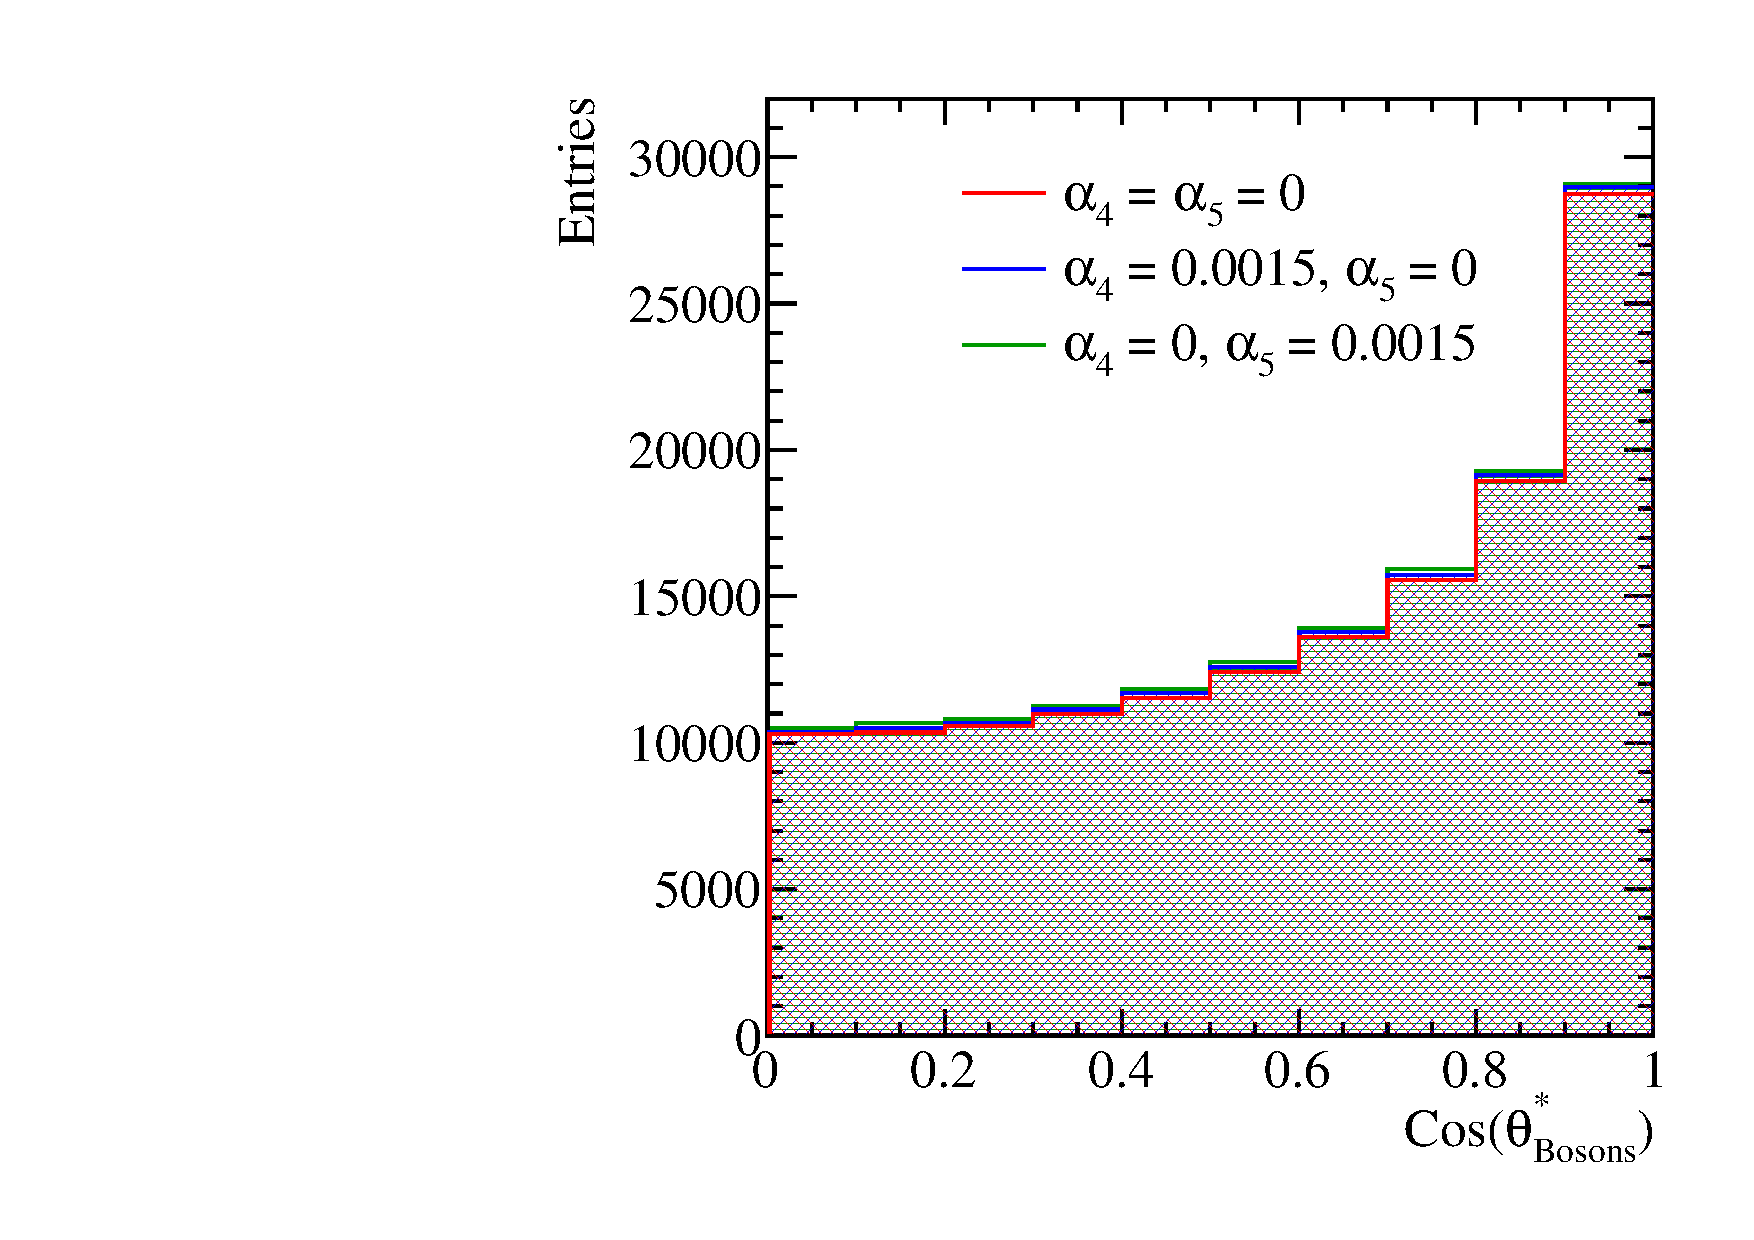
\includegraphics[width=0.5\textwidth]{PhysicsAnalysis/Plots/SensitiveDistributions/CosThetaStarSynBosons_SPFOs_kt_0p70_3000GeV.pdf}}
\caption[Sensitivity of $\text{cos}\theta^{8}_{Bosons}$ to the anomalous gauge couplings $\alpha_{4}$ and $\alpha_{5}$ at 1.4 and 3 TeV.]{Sensitivity of $\text{cos}\theta^{*}_{Bosons}$ to anomalous couplings at 1.4 and 3 TeV. The jet algorithm used for this example was the longitudinally invariant kt algorithm with an R parameter of 0.7. This sample corresponds to pure signal of hadronic decays in vector boson scattering i.e. \nu{\nu}qqqq.}
\label{fig:costhetastarbosons}
\end{figure}

At 1.4 TeV event weights were produced from Whizard stepping along $\alpha_{4}$ and $\alpha_{5}$ in steps of 0.01 ranging from -0.07 to 0.07 as shown in figure \ref{fig:eventweights1400raw}, however, to produce a smooth $\chi^{2}$ contour much finer sampling is needed.  While it is feasible to generate new event weights in Whizard for any pair of $\alpha_{4}$ and $\alpha_{5}$ it is time consuming making it impractical for this analysis.  To overcome this difficulty bicubic interpolation is applied between these points to allow for the extract of event weights anywhere within the range -0.05 to 0.05.  As figure \ref{fig:eventweights1400interpolated} shows the interpolated surface proves to be a good fit to the data produced from the generator in that it is smooth and continuous.  

Similarly at 3 TeV the same procedure was used but stepping occurs in steps of 0.001 ranging from -0.007 to 0.007 in both $\alpha_{4}$ and $\alpha_{5}$.  These ranges proved to be sufficient for the contours of interest for the CLIC sensitivity analysis at this energy.

\begin{figure}
\centering
\subfloat[]{\label{fig:weight1}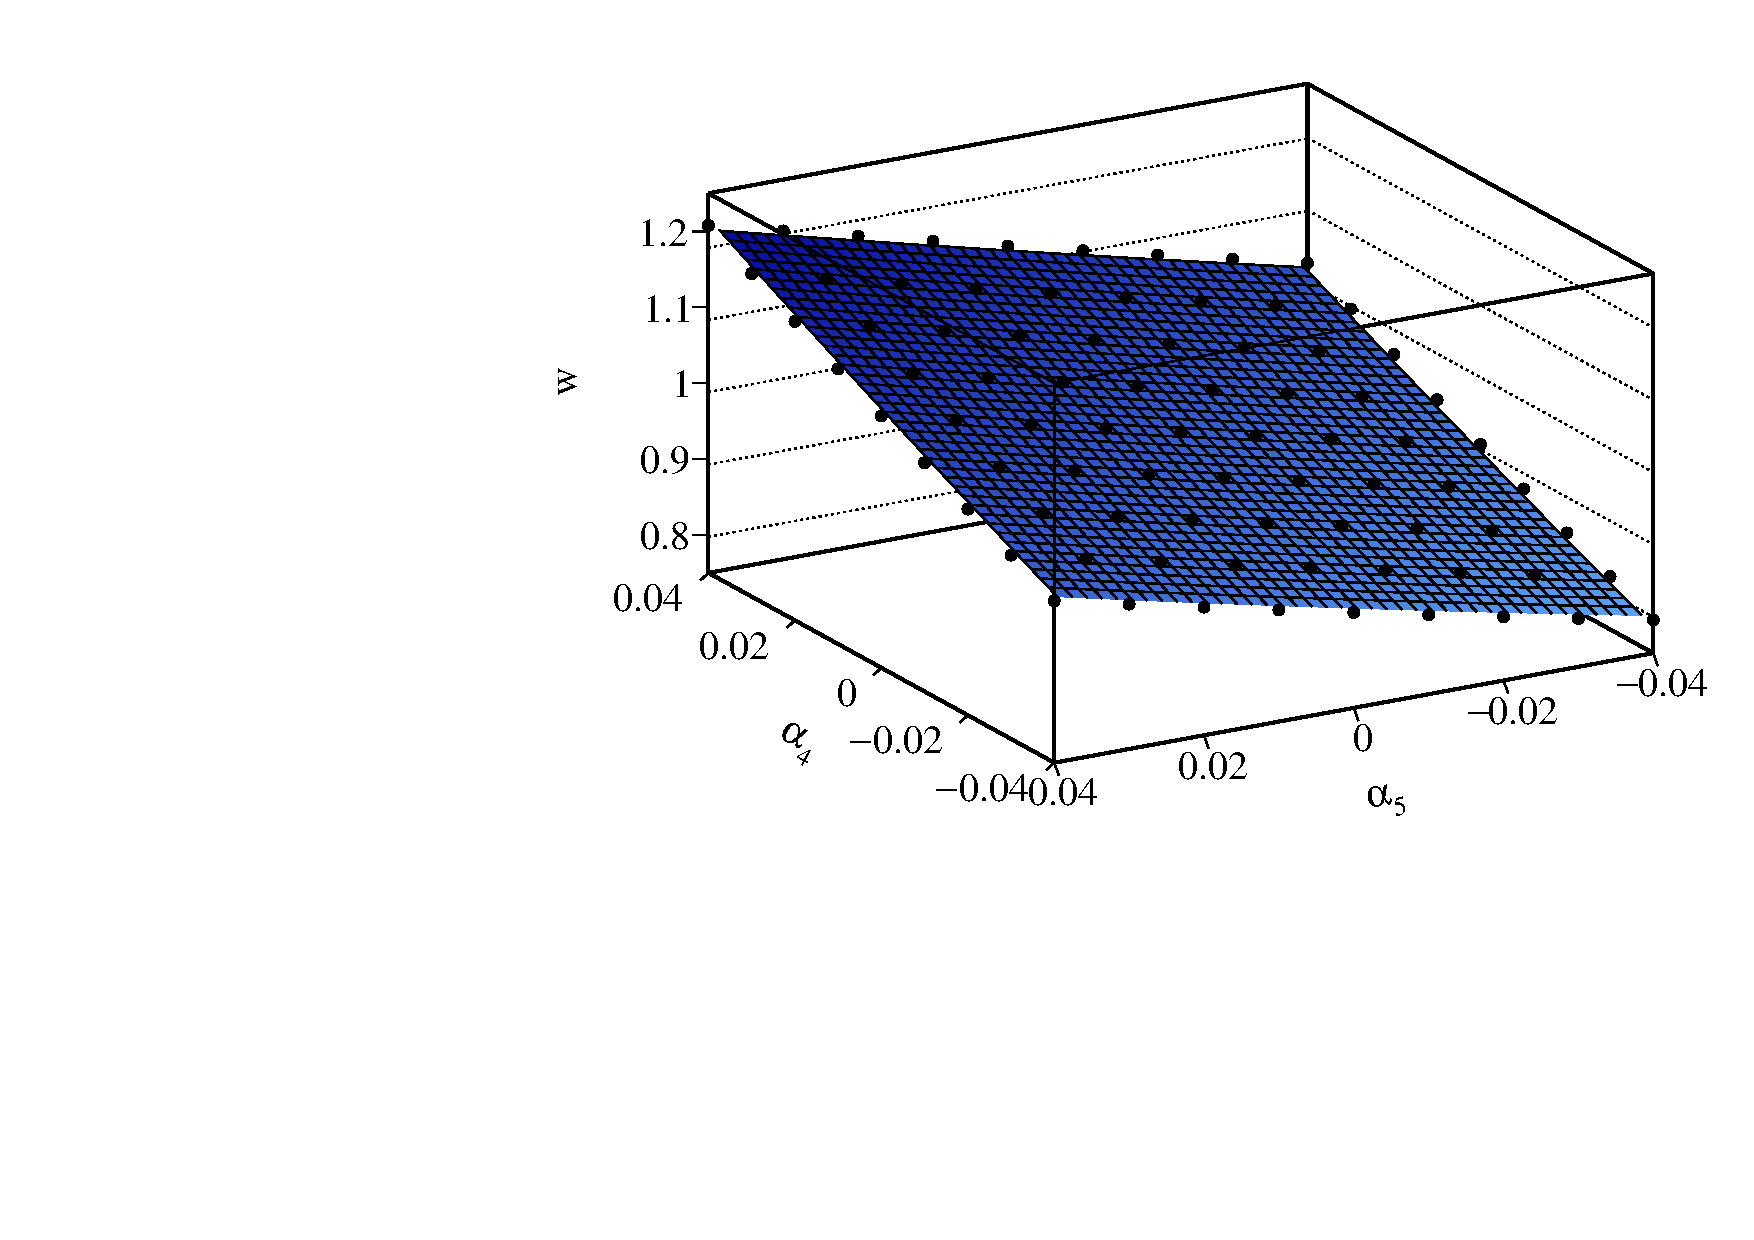
\includegraphics[width=0.5\textwidth]{PhysicsAnalysis/Plots/EventWeights/1400GeV/EventWeightsForEvent100001009_1400GeV_SPFOs_kt_0p70_10Bins_Start_0_End_10_1400GeV_Interpolated.pdf}}
\subfloat[]{\label{fig:weight2}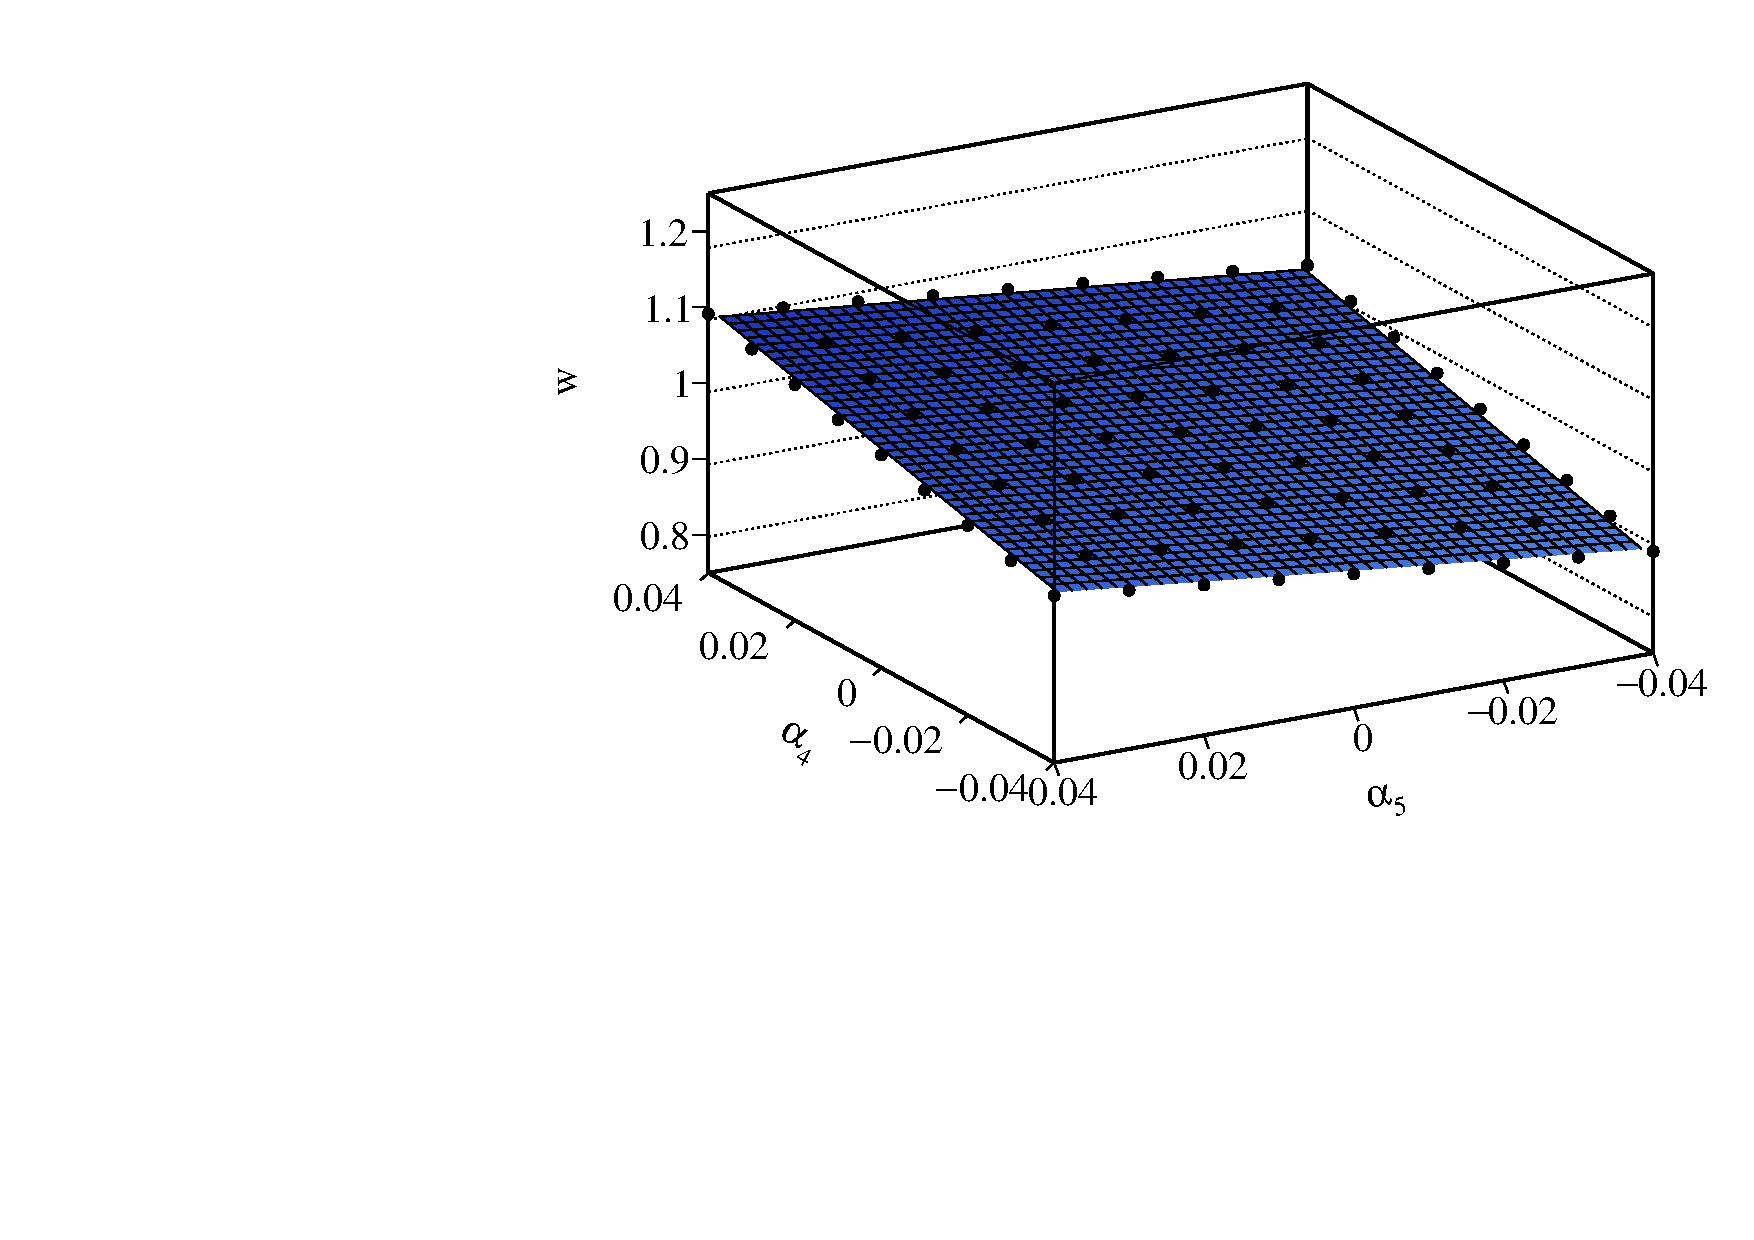
\includegraphics[width=0.5\textwidth]{PhysicsAnalysis/Plots/EventWeights/1400GeV/EventWeightsForEvent100001014_1400GeV_SPFOs_kt_0p70_10Bins_Start_0_End_10_1400GeV_Interpolated.pdf}} \hfill
\subfloat[]{\label{fig:weight3}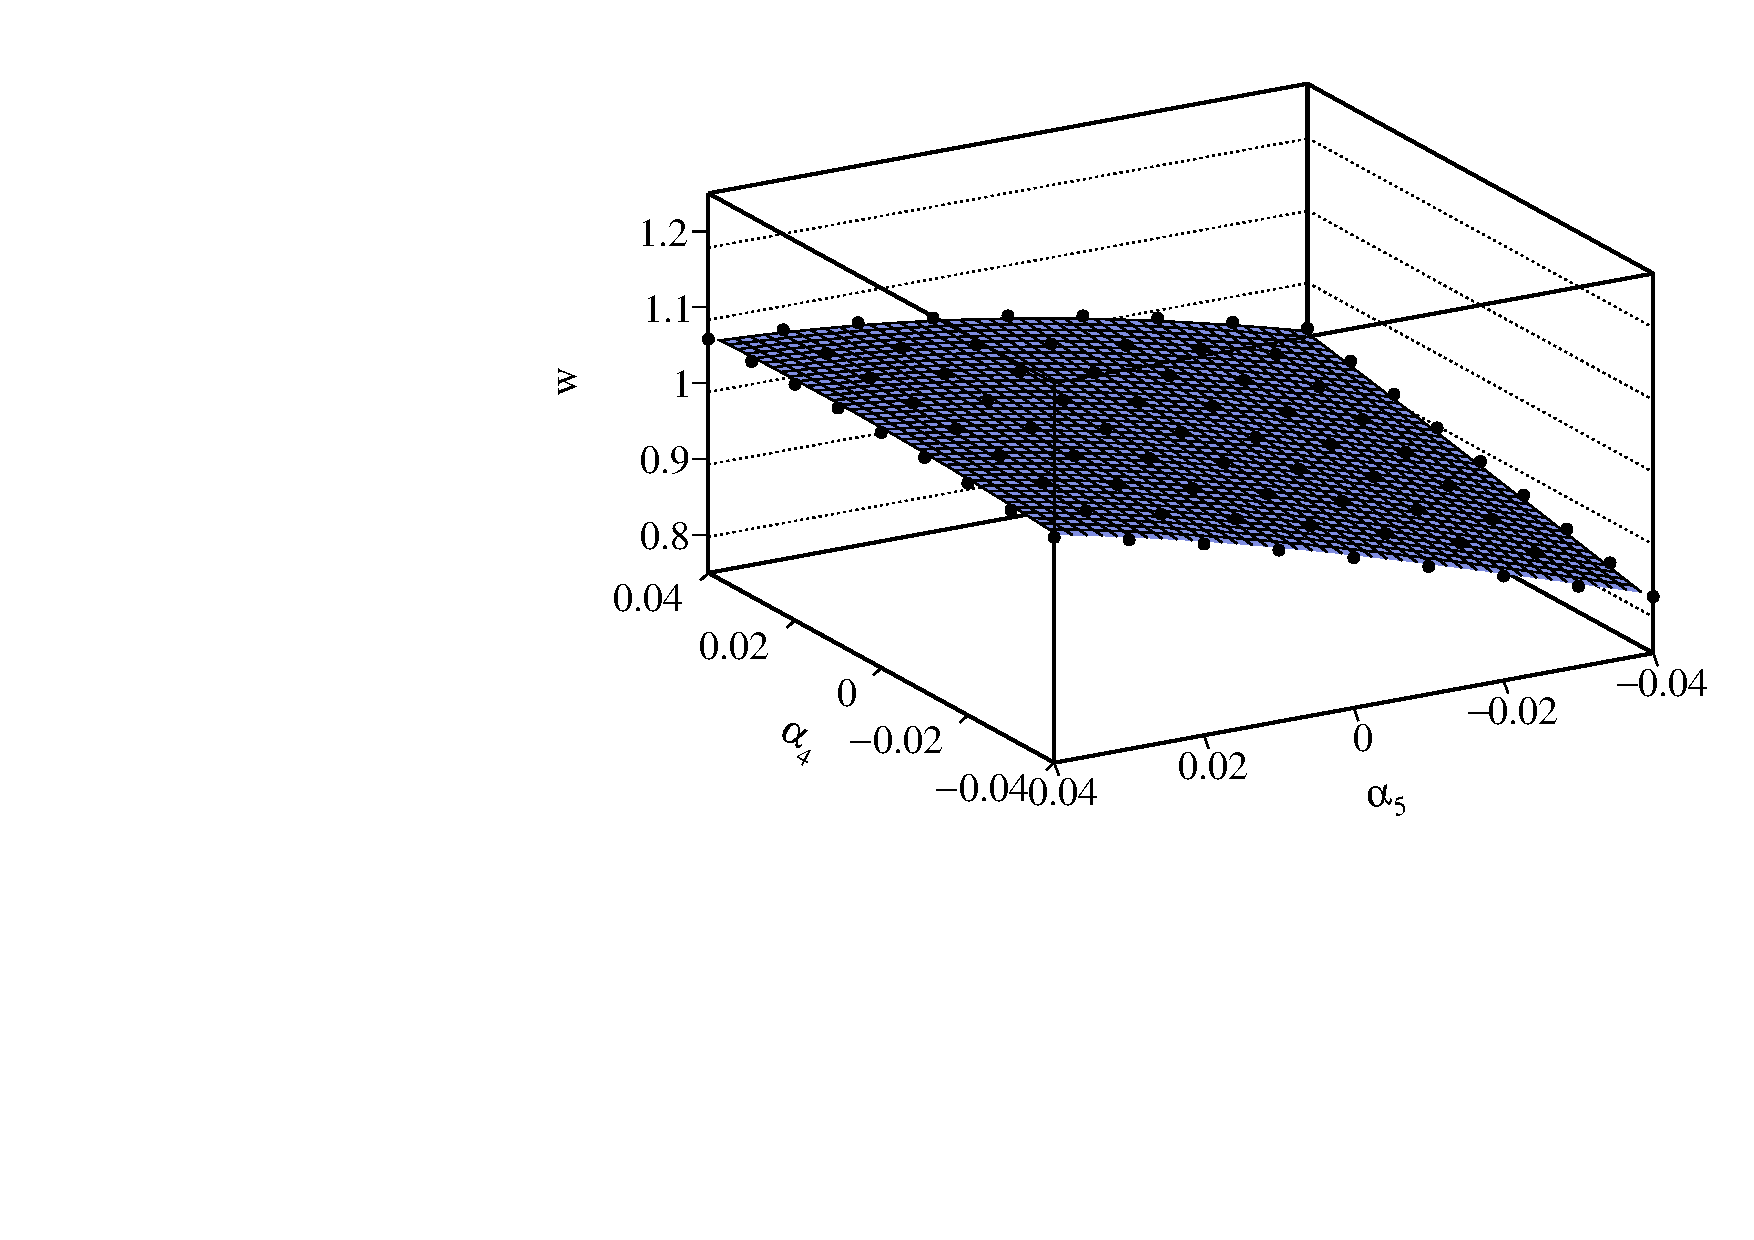
\includegraphics[width=0.5\textwidth]{PhysicsAnalysis/Plots/EventWeights/1400GeV/EventWeightsForEvent100001044_1400GeV_SPFOs_kt_0p70_10Bins_Start_0_End_10_1400GeV_Interpolated.pdf}}
\subfloat[]{\label{fig:weight4}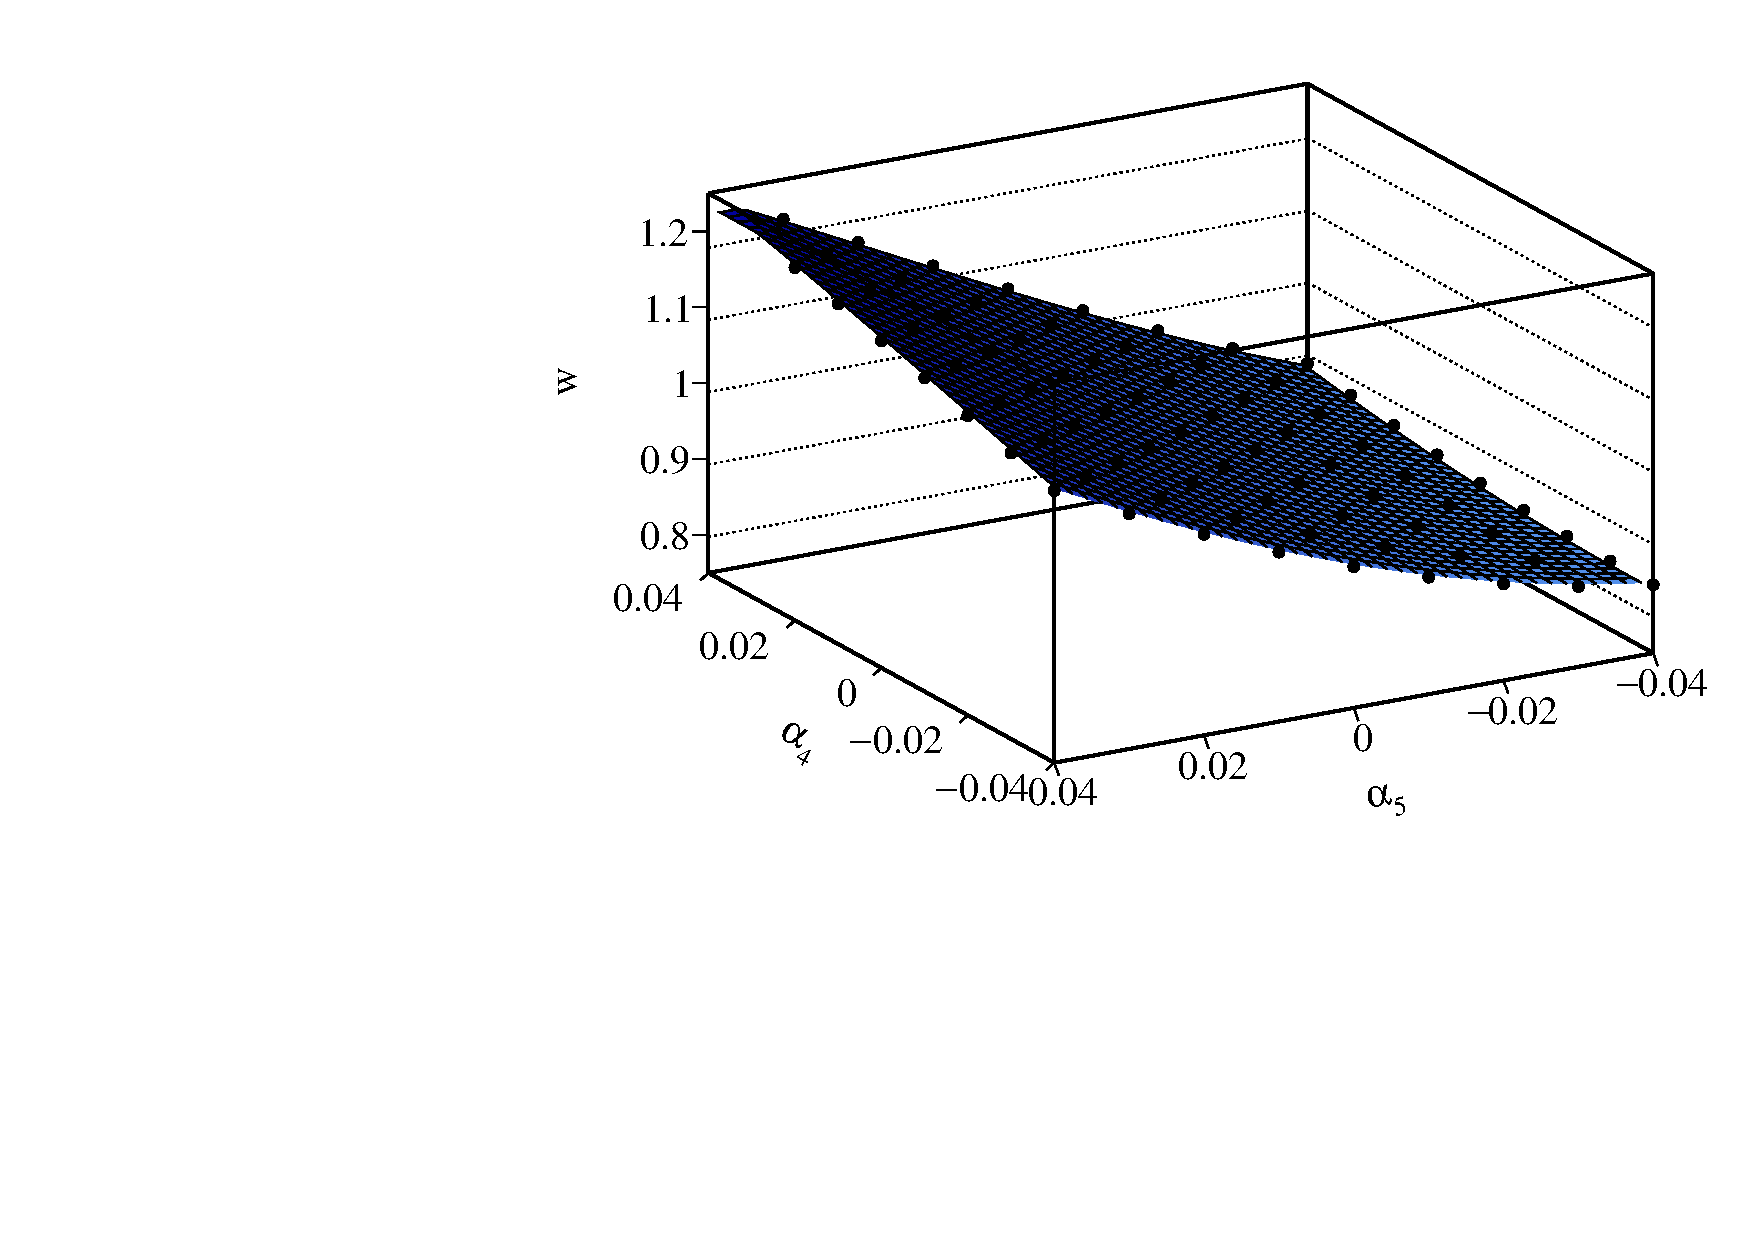
\includegraphics[width=0.5\textwidth]{PhysicsAnalysis/Plots/EventWeights/1400GeV/EventWeightsForEvent100001051_1400GeV_SPFOs_kt_0p70_10Bins_Start_0_End_10_1400GeV_Interpolated.pdf}}
\caption[Event weights from Whizard for 1.4TeV \nu{\nu}qqqq final state events with interpolated surface.]{A selection of plots showing how the event weight changes when varying the anomalous couplings $\alpha_{4}$ and $\alpha_{5}$ for 1.4TeV \nu{\nu}qqqq final state events.  The hollow circles show the event weight produced from the generator while the surface shown is found using bicubic interpolation between those points.}
\label{fig:eventweights1400interpolated}
\end{figure}

Using these interpolated surfaces for the event weights, distribution of $\text{cos}\theta^{*}_{Jets}$ were produced stepping across $\alpha_{4}$ and $\alpha_{5}$ in steps of 0.0001 at 1.4 TeV and 0.00001 at 3 TeV.  Each distribution was converted into a value of $\chi^{2}$ using the following formula:

\begin{equation}
\chi^{2} = \Sigma_{i} \frac{(O_{i} - E_{i})^{2}}{E_{i}}
\end{equation}

where $O_{i}$ is the observed bin content for bin i in the distribution with non-zero $\alpha_{4}$ and $\alpha_{5}$ and $E_{i}$ is the expected bin content for bin i in the distribution with zero $\alpha_{4}$ and $\alpha_{5}$ i.e. the standard model expected value.

\section{Optimisation of Jet Reconstruction}

The jet algorithm used for this analysis is the longitudinally invariant kt algorithm as described in section \ref{sec:jetpairing}.  The parameter choices under consideration for optimisation are the R parameter, used in the kt algorithm definition, used and the PFO selection.  

A number of cuts \cite{arXiv:1209.4039} are applied to the transverse momenta and the time of the PFOs produced by PandoraPFA to reduce the PFOs into a subset that are believed to originate from the desired interaction in an attempt to veto the overlaid $\gamma\gamma \rightarrow \text{Hadron}$ background events.  Different options for these cuts  give rise to the tight, default and loose selected PFOs that are considered in this optimisation.  

The optimal sensitivity is achieved for either loose selected PFOs with an R parameter of 0.7 or default selected PFOs with an R parameter of 0.9 as can be seen from tables \ref{table:precisiona4signaljetalgo} and \ref{table:precisiona5signaljetalgo}.  As a tie breaker between these options the separation power, the fraction of events misidentified as either arising from a WW pair or a ZZ pair, was considered.  Again performance was similar, but there was a slight preference towards the use of selected PFOs and an R parameter of 0.9.  While not used in the primary analysis the separation of samples into WW and ZZ events is important for an extension analysis found in section BLAH.

The optimal contours can be found in figure \ref{fig:chi2jetalgoideal1400GeV} and the optimal 1D plot used to produce the errors references in the tables \ref{table:precisiona4signaljetalgo} and \ref{table:precisiona5signaljetalgo} can be found in figures \ref{fig:a4chi2jetalgoideal1400GeV} and \ref{fig:a5chi2jetalgoideal1400GeV} respectively.  All other contours and plots for this optimisation can be found in the appendices.  

\begin{table}[h!]
\centering
\begin{tabular}{l l l l}
\hline
PFO Selection & Tight Selected PFOs & Selected PFOs & Loose Selected PFOs \\ 
R Parameter & & & \\ 
\hline
0.7 & $-0.0039$ $+0.0050$ & $-0.0038$ $+0.0050$ & $-0.0037$ $+0.0046$ \\
0.9 & $-0.0041$ $+0.0051$ & $-0.0038$ $+0.0046$ & $-0.0038$ $+0.0048$ \\
1.1 & $-0.0041$ $+0.0051$ & $-0.0039$ $+0.0050$ & $-0.0040$ $+0.0050$ \\
\hline
\end{tabular}
\caption[$1\sigma$ precision on measurement of $\alpha_{4}$ for different jet reconstruction parameters considering pure signal.]{Precision on measurement of $\alpha_{4}$ for different jet reconstruction parameters considering pure signal and applying a $\chi^{2}$ fit to $\text{cos}\theta^{*}_{Jets}$.}
\label{table:precisiona4signaljetalgo}
\end{table}

\begin{table}[h!]
\centering
\begin{tabular}{l l l l}
\hline
PFO Selection & Tight Selected PFOs & Selected PFOs & Loose Selected PFOs \\ 
R Parameter & & & \\ 
\hline
0.7 & $-0.0027$ $+0.0031$ & $-0.0027$ $+0.0032$ & $-0.0025$ $+0.0030$ \\
0.9 & $-0.0028$ $+0.0032$ & $-0.0026$ $+0.0030$ & $-0.0026$ $+0.0030$ \\
1.1 & $-0.0028$ $+0.0032$ & $-0.0027$ $+0.0032$ & $-0.0028$ $+0.0031$ \\
\hline
\end{tabular}
\caption[$1\sigma$ precision on measurement of $\alpha_{5}$ for different jet reconstruction parameters considering pure signal.]{Precision on measurement of $\alpha_{5}$ for different jet reconstruction parameters considering pure signal and applying a $\chi^{2}$ fit to $\text{cos}\theta^{*}_{Jets}$.}
\label{table:precisiona5signaljetalgo}
\end{table}

\begin{figure}
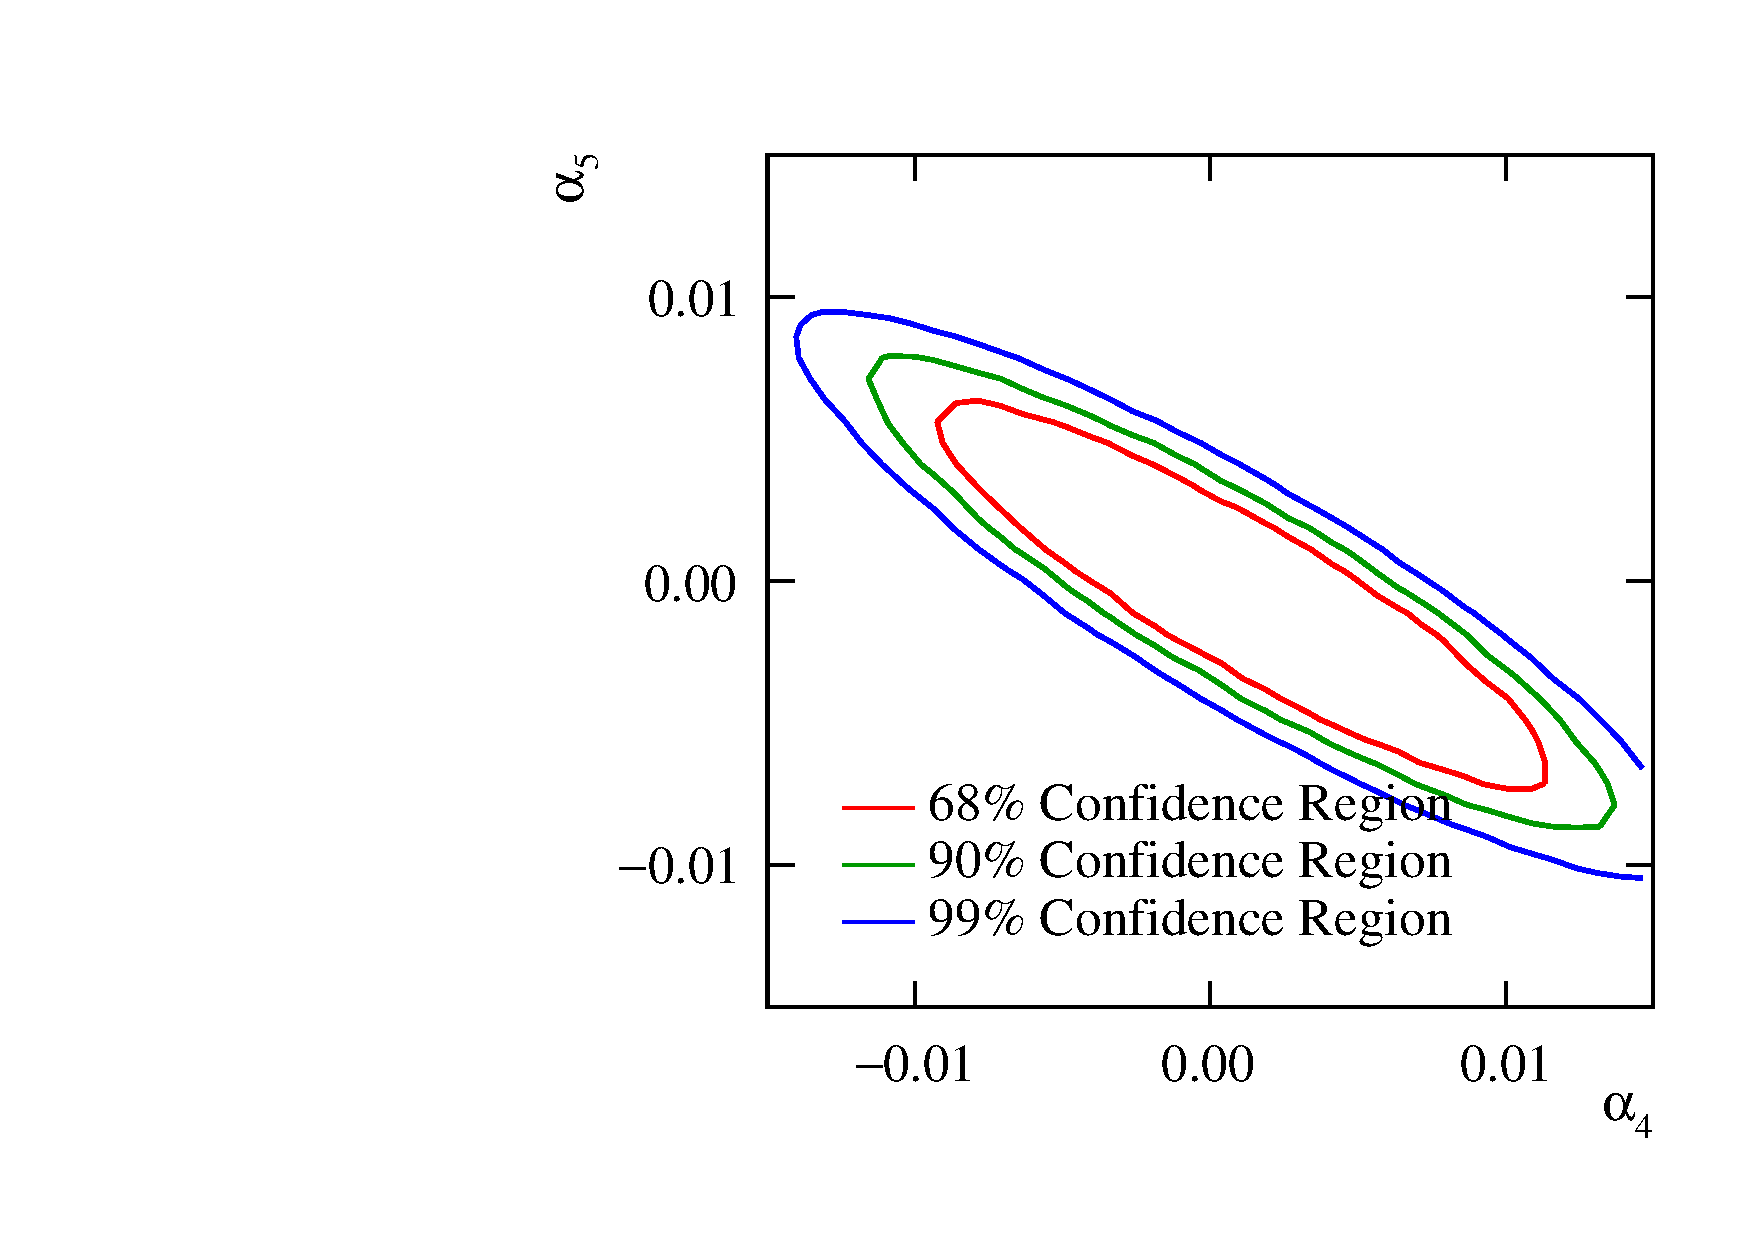
\includegraphics[width=0.75\textwidth]{PhysicsAnalysis/Plots/Chi2ContoursOptimisation/1400GeV/KtSPFOsR0p90.pdf}
\caption[$\chi^{2}$ Sensitivity contours for the $\text{qqqq}\nu\nu$ final state arising from a fit to $\text{cos}\theta^{*}_{\text{Jets}}$ at 1.4 TeV for the optimal jet reconstruction parameters.]{$\chi^{2}$ Sensitivity contours for the $\text{qqqq}\nu\nu$ final state arising from a fit to $\text{cos}\theta^{*}_{\text{Jets}}$ at 1.4 TeV for the optimal jet reconstruction parameters.}
\label{fig:chi2jetalgoideal1400GeV}
\end{figure}

\begin{figure}
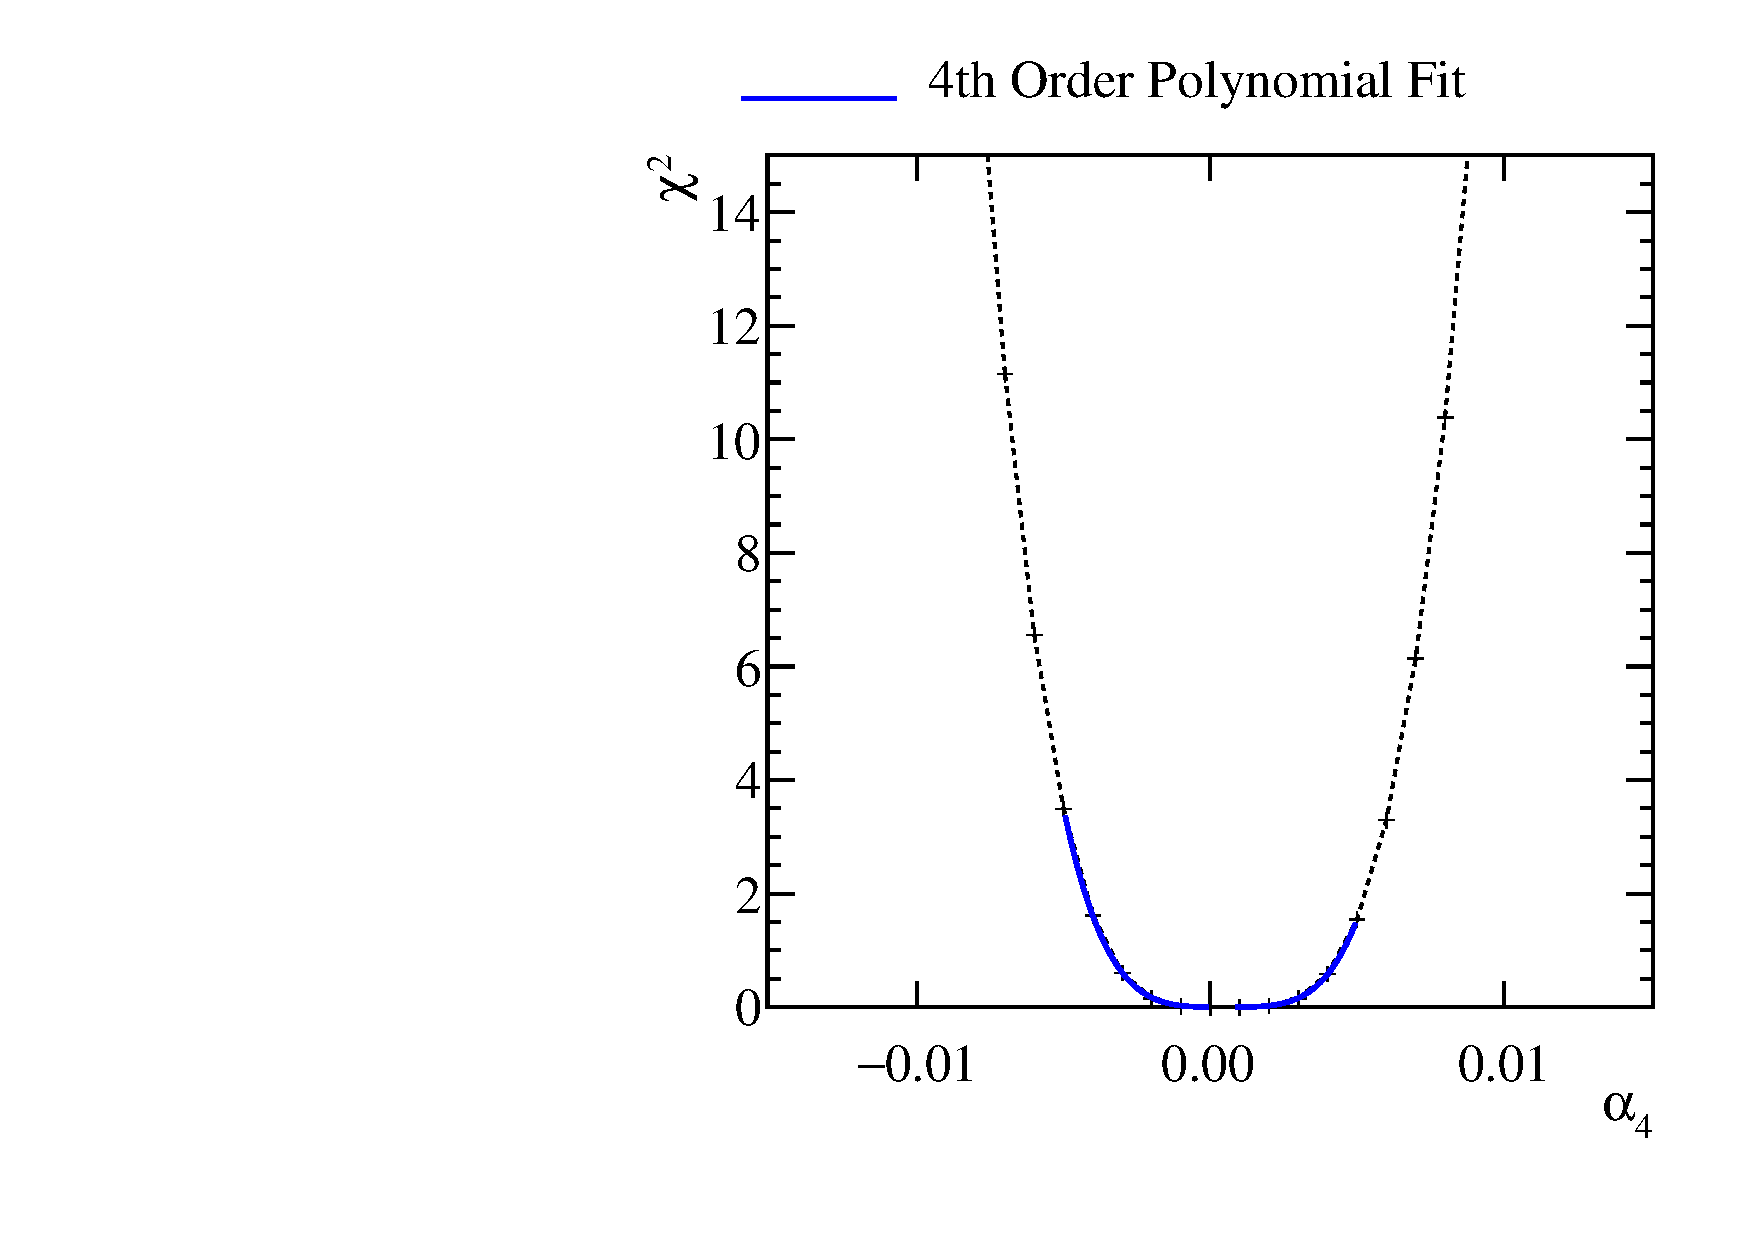
\includegraphics[width=0.75\textwidth]{PhysicsAnalysis/Plots/Chi2ContoursOptimisation/1400GeV/KtSPFOsR0p90_alpha4.pdf}
\caption[$\chi^{2}$ as a function of $\alpha_{4}$ assuming $\alpha_{5} = 0$ for the $\text{qqqq}\nu\nu$ final state arising from a fit to $\text{cos}\theta^{*}_{\text{Jets}}$ at 1.4 TeV for the optimal jet reconstruction parameters.]{$\chi^{2}$ as a function of $\alpha_{4}$ assuming $\alpha_{5} = 0$ for the $\text{qqqq}\nu\nu$ final state arising from a fit to $\text{cos}\theta^{*}_{\text{Jets}}$ at 1.4 TeV for the optimal jet reconstruction parameters.}
\label{fig:a4chi2jetalgoideal1400GeV}
\end{figure}

\begin{figure}
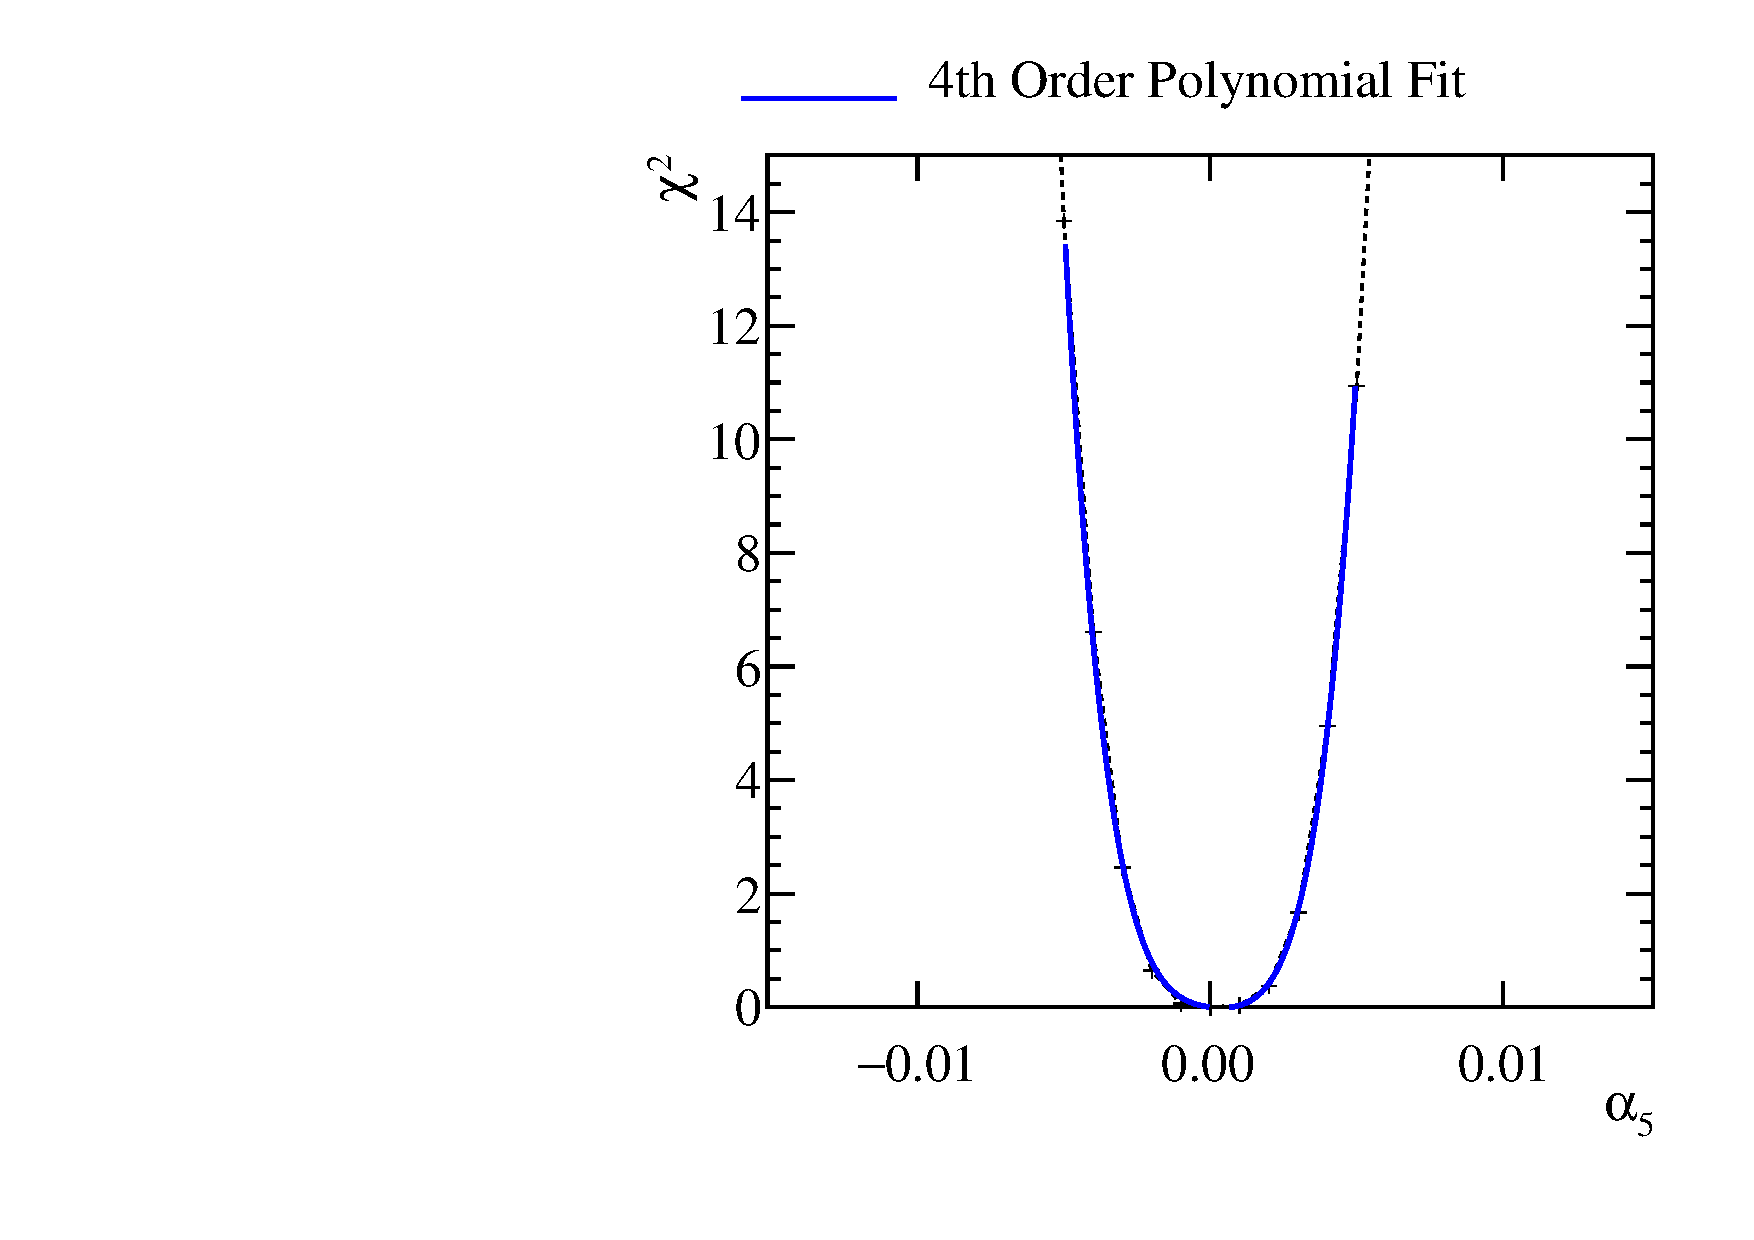
\includegraphics[width=0.75\textwidth]{PhysicsAnalysis/Plots/Chi2ContoursOptimisation/1400GeV/KtSPFOsR0p90_alpha5.pdf}
\caption[$\chi^{2}$ as a function of $\alpha_{5}$ assuming $\alpha_{4} = 0$ for the $\text{qqqq}\nu\nu$ final state arising from a fit to $\text{cos}\theta^{*}_{\text{Jets}}$ at 1.4 TeV for the optimal jet reconstruction parameters.]{$\chi^{2}$ as a function of $\alpha_{5}$ assuming $\alpha_{4} = 0$ for the $\text{qqqq}\nu\nu$ final state arising from a fit to $\text{cos}\theta^{*}_{\text{Jets}}$ at 1.4 TeV for the optimal jet reconstruction parameters.}
\label{fig:a5chi2jetalgoideal1400GeV}
\end{figure}

\section{Event Selection}

As discussed earlier the signal events for this analysis contain the \nu{\nu}qqqq final state. The processes to be considered in this analysis alongside the signal are events that would topologically look similar to signal in the detector. This includes events that could be confused with 4 jet events with missing energy, while excluding those events with large numbers of high energy leptons that could be vetoed easily during the analysis stage. In full the list includes:

\begin{table}[h!]
\centering
\begin{tabular}{ l l l}
\hline
Final State & Cross Section 1.4 TeV [fb] & Cross Section 3 TeV [fb]  \\ 
\hline
$\text{e}^{+}\text{e}^{-} \rightarrow \nu{\nu}\text{qqqq}$ & 24.7 & 71.5 \\
$\text{e}^{+}\text{e}^{-} \rightarrow \text{l}\nu\text{qqqq}$ & 110.4 & 106.6 \\
$\text{e}^{+}\text{e}^{-} \rightarrow \text{llqqqq}$ & 62.1 & 169.3 \\
$\text{e}^{+}\text{e}^{-} \rightarrow \text{qqqq}$ & 1245.1 & 546.5 \\
$\text{e}^{+}\text{e}^{-} \rightarrow \nu{\nu}\text{qq}$ & 787.7 & 546.5 \\
$\text{e}^{+}\text{e}^{-} \rightarrow \text{l}\nu\text{qq}$ & 4309.7 & 5560.9 \\
$\text{e}^{+}\text{e}^{-} \rightarrow \text{llqq}$ & 2725.8 & 3319.6 \\
$\text{e}^{+}\text{e}^{-} \rightarrow \text{qq}$ & 4009.5 & 2948.9 \\
$\gamma_{\text{EPA}}\text{e}^{-} \rightarrow \text{qqqq}\text{e}^{-}$ & 287.1 & 287.8 \\
$\gamma_{\text{BS}}\text{e}^{-} \rightarrow \text{qqqq}\text{e}^{-}$ & 1160.7 & 1268.6 \\
$\text{e}^{+}\gamma_{\text{EPA}} \rightarrow \text{qqqq}\text{e}^{+}$ & 286.9 & 287.8 \\
$\text{e}^{+}\gamma_{\text{BS}} \rightarrow \text{qqqq}\text{e}^{+}$ & 1156.3 & 1267.3 \\
$\gamma_{\text{EPA}}\text{e}^{-} \rightarrow \text{qqqq}\nu$ & 32.6 & 54.2 \\
$\gamma_{\text{BS}}\text{e}^{-} \rightarrow \text{qqqq}\nu$ & 136.9 & 262.5 \\
$\text{e}^{+}\gamma_{\text{EPA}} \rightarrow \text{qqqq}\nu$ & 32.6 & 54.2 \\
$\text{e}^{+}\gamma_{\text{BS}} \rightarrow \text{qqqq}\nu$ & 136.4 & 262.3 \\
$\gamma_{\text{EPA}}\gamma_{\text{EPA}} \rightarrow \text{qqqq}$ & 753.0 & 402.7 \\
$\gamma_{\text{EPA}}\gamma_{\text{BS}} \rightarrow \text{qqqq}$ & 4034.8 & 2423.1 \\
$\gamma_{\text{BS}}\gamma_{\text{EPA}} \rightarrow \text{qqqq}$ & 4018.7 & 2420.6 \\
$\gamma_{\text{BS}}\gamma_{\text{BS}} \rightarrow \text{qqqq}$ & 21406.2 & 13050.3 \\
\hline
\end{tabular}
\caption[]{Cross sections of signal and background processes at 1.4 and 3 TeV. In the above table q $\in$ u, $\bar{\text{u}}$, d, $\bar{\text{d}}$, s, $\bar{\text{s}}$, c, $\bar{\text{c}}$, b or $\bar{\text{b}}$ while l $\in$ $\text{e}^{\pm}$, $\mu^{\pm}$ or $\tau^{\pm}$ and $\nu$ $\in$ $\nu_{e}$, $\nu_{\mu}$ and $\nu_{\tau}$.  The subscript EPA or BS for the incoming photons indicate whether the photon is generated from the equivalent photon approximation or beamstrahlung.}
\label{table:crosssectionfull}
\end{table}

Equivalent photon approximation processes models interactions of the electric field of the incoming electrons and positrons with their corresponding antiparticles at the collision point. In such interactions the electric fields of the charged particles are approximated as photons hence the name. The beamstrahlung processes model the collision of a photon radiated off a charged particle with the corresponding bunch incoming lepton. Photons are radiated from the incoming charged leptons as the bunches carrying the leptons are very small producing very large electromagnetic fields. Interactions with the charged leptons and these fields yields the beamstrahlung photons. The energy spectrum of the incoming particles for CLIC at the relevant operating energy is used to model the energy of the incoming photons. Included in these cases are the photon-photon interactions from photons appearing from the EPA and beamstrahlung processes.

A dominant background process appearing at CLIC is $\gamma\gamma \rightarrow \text{Hadron}$. Example Feynman diagrams for such processes is shown in figure ??. Unlike the majority of other background processes, such as incoherent pair production of $\text{e}^{+}\text{e}^{-}$ pairs from beamstrahlung photons and beam halo muons from interactions of the beam with particles outside the detector, the $\gamma\gamma \rightarrow \text{Hadron}$ processes have a large transverse momentum and cannot be vetoed with a simple transverse momentum cut. To account for this non negligible background $\gamma\gamma \rightarrow \text{Hadron}$ events are overlaid onto CLIC samples. The number of events overlaid per event is drawn from a Poisson with a mean of 3.2 for 3 TeV and 1.3 for 1.4 TeV samples. Maybe include CDR plot on page 54.

\subsection{Pre Selection - 1.4 TeV}

The primary selection of the \nu{\nu}qqqq signal will be done using a multivariate analysis, however, in an attempt to veto trivial backgrounds a simple cut based preselection is applied. Cuts are applied to the transverse momentum, invariant mass of the visible system and the number of isolated leptons. The raw distributions of these variables is
shown in figures \ref{fig:preselection1}, \ref{fig:preselection2} and \ref{fig:preselection3}. Based on these distributions the following cuts were applied:

\begin{itemize}
\item Transverse momentum > 100 GeV. This cut is effective due to the presence of missing energy in the form of neutrinos in the signal final state.
\item Visible mass of the system > 200 GeV. This cut is effective for accounting for the missing energy of the neutrinos in the final state along the longitudinal direction of the detector instead.
\item Number of isolated leptons = 0. This cut vetos a large number of events with leptons in the final state.
The effect of these preselection cuts can be found in table 1.3. While a large fraction of the signal events are lost through these cuts, particularly the transverse momentum cuts, a much large fraction of background events are removed justifying the cut.
\end{itemize}

The event numbers for the signal and background are shown in table \ref{table:cutflow1400GeV} as these cuts are cumulatively applied.  These numbers are normalised to the correct luminosity for CLIC running at 1.4 TeV.  

As referenced in section  <- Iso lep finder good at vetoing other sensitive events 

\begin{table}[h!]
\centering
\begin{tabular}{ l l l l l}
\hline
Final State & Raw Event  & $p_{T}$ > 100 GeV & $p_{T}$ > 100 GeV \& & $p_{T}$ > 100 GeV \& \\ 
& Numbers & & $M_{\text{Vis}}$ > 200 GeV & $M_{\text{Vis}}$ > 200 GeV \&\\ 
& & & & $N_{\text{Isolated Leptons}}$ = 0\\ 
\hline
$\text{e}^{+}\text{e}^{-} \rightarrow \nu{\nu}\text{qqqq}$ & 37,050 & 23,782 & 21,091 & 21,034 \\
$\text{e}^{+}\text{e}^{-} \rightarrow \text{l}\nu\text{qqqq}$ & 165,600 & 81,631 & 80,827 & 42,332 \\
$\text{e}^{+}\text{e}^{-} \rightarrow \text{llqqqq}$ & 93,150 & 1,154 & 1,142 & 710 \\
$\text{e}^{+}\text{e}^{-} \rightarrow \text{qqqq}$ & 1,867,631 & 6,755 & 6,742 & 6,729 \\
$\text{e}^{+}\text{e}^{-} \rightarrow \nu{\nu}\text{qq}$ & 1,181,218 & 514,701 & 49,692 & 49,586 \\
$\text{e}^{+}\text{e}^{-} \rightarrow \text{l}\nu\text{qq}$ & 6,463,852 & 2,002,405 & 1,258,172 & 568,450 \\
$\text{e}^{+}\text{e}^{-} \rightarrow \text{llqq}$ & 4,088,143 & 7,656 & 7,263 & 5,651 \\
$\text{e}^{+}\text{e}^{-} \rightarrow \text{qq}$ & 6,010,154 & 34,123 & 33,679 & 33,605 \\
$\gamma_{\text{EPA}}\text{e}^{-} \rightarrow \text{qqqq}\text{e}^{-}$ & 430,643 & 2,301 & 2,294 & 762 \\
$\gamma_{\text{BS}}\text{e}^{-} \rightarrow \text{qqqq}\text{e}^{-}$ & 1,741,050 & 1,773 & 1,688 & 1,294 \\
$\text{e}^{+}\gamma_{\text{EPA}} \rightarrow \text{qqqq}\text{e}^{+}$ & 430,344 & 2,787 & 2,774 & 1,057 \\
$\text{e}^{+}\gamma_{\text{BS}} \rightarrow \text{qqqq}\text{e}^{+}$ & 1,734,450 & 814 & 784 & 552 \\
$\gamma_{\text{EPA}}\text{e}^{-} \rightarrow \text{qqqq}\nu$ & 48,893 & 17,468 & 13,558 & 8,895 \\
$\gamma_{\text{BS}}\text{e}^{-} \rightarrow \text{qqqq}\nu$ & 205,326 & 75,429 & 48,648 & 48,023 \\
$\text{e}^{+}\gamma_{\text{EPA}} \rightarrow \text{qqqq}\nu$ & 48,893 & 17,656 & 13,588 & 8,951 \\
$\text{e}^{+}\gamma_{\text{BS}} \rightarrow \text{qqqq}\nu$ & 204,581 & 74,890 & 48,457 & 47,903 \\
$\gamma_{\text{EPA}}\gamma_{\text{EPA}} \rightarrow \text{qqqq}$ & 1,129,459 & 3,126 & 3,018 & 1,421 \\
$\gamma_{\text{EPA}}\gamma_{\text{BS}} \rightarrow \text{qqqq}$ & 6,052,200 & 7,205 & 7,059 & 5,531 \\
$\gamma_{\text{BS}}\gamma_{\text{EPA}} \rightarrow \text{qqqq}$ & 6,027,979 & 5,187 & 5,116 & 3,197 \\
$\gamma_{\text{BS}}\gamma_{\text{BS}} \rightarrow \text{qqqq}$ & 32,109,300 & 4,421 & 4,421 & 3,617 \\
\hline
\end{tabular}
\caption[Impact of preselection cuts on signal and background at 1.4 TeV.]{Impact of preselection cuts on signal and background at 1.4 TeV.  $p_{T}$ is the transverse momentum of the event,  $M_{\text{Vis}}$ is the visible mass and $N_{\text{Isolated Leptons}}$ is the number of isolated leptons in the event.  In the above table q $\in$ u, $\bar{\text{u}}$, d, $\bar{\text{d}}$, s, $\bar{\text{s}}$, c, $\bar{\text{c}}$, b or $\bar{\text{b}}$ while l $\in$ $\text{e}^{\pm}$, $\mu^{\pm}$ or $\tau^{\pm}$ and $\nu$ $\in$ $\nu_{e}$, $\nu_{\mu}$ and $\nu_{\tau}$.  The subscript EPA or BS for the incoming photons indicate whether the photon is generated from the equivalent photon approximation or beamstrahlung.}
\label{table:cutflow1400GeV}
\end{table}

\begin{figure}
\centering
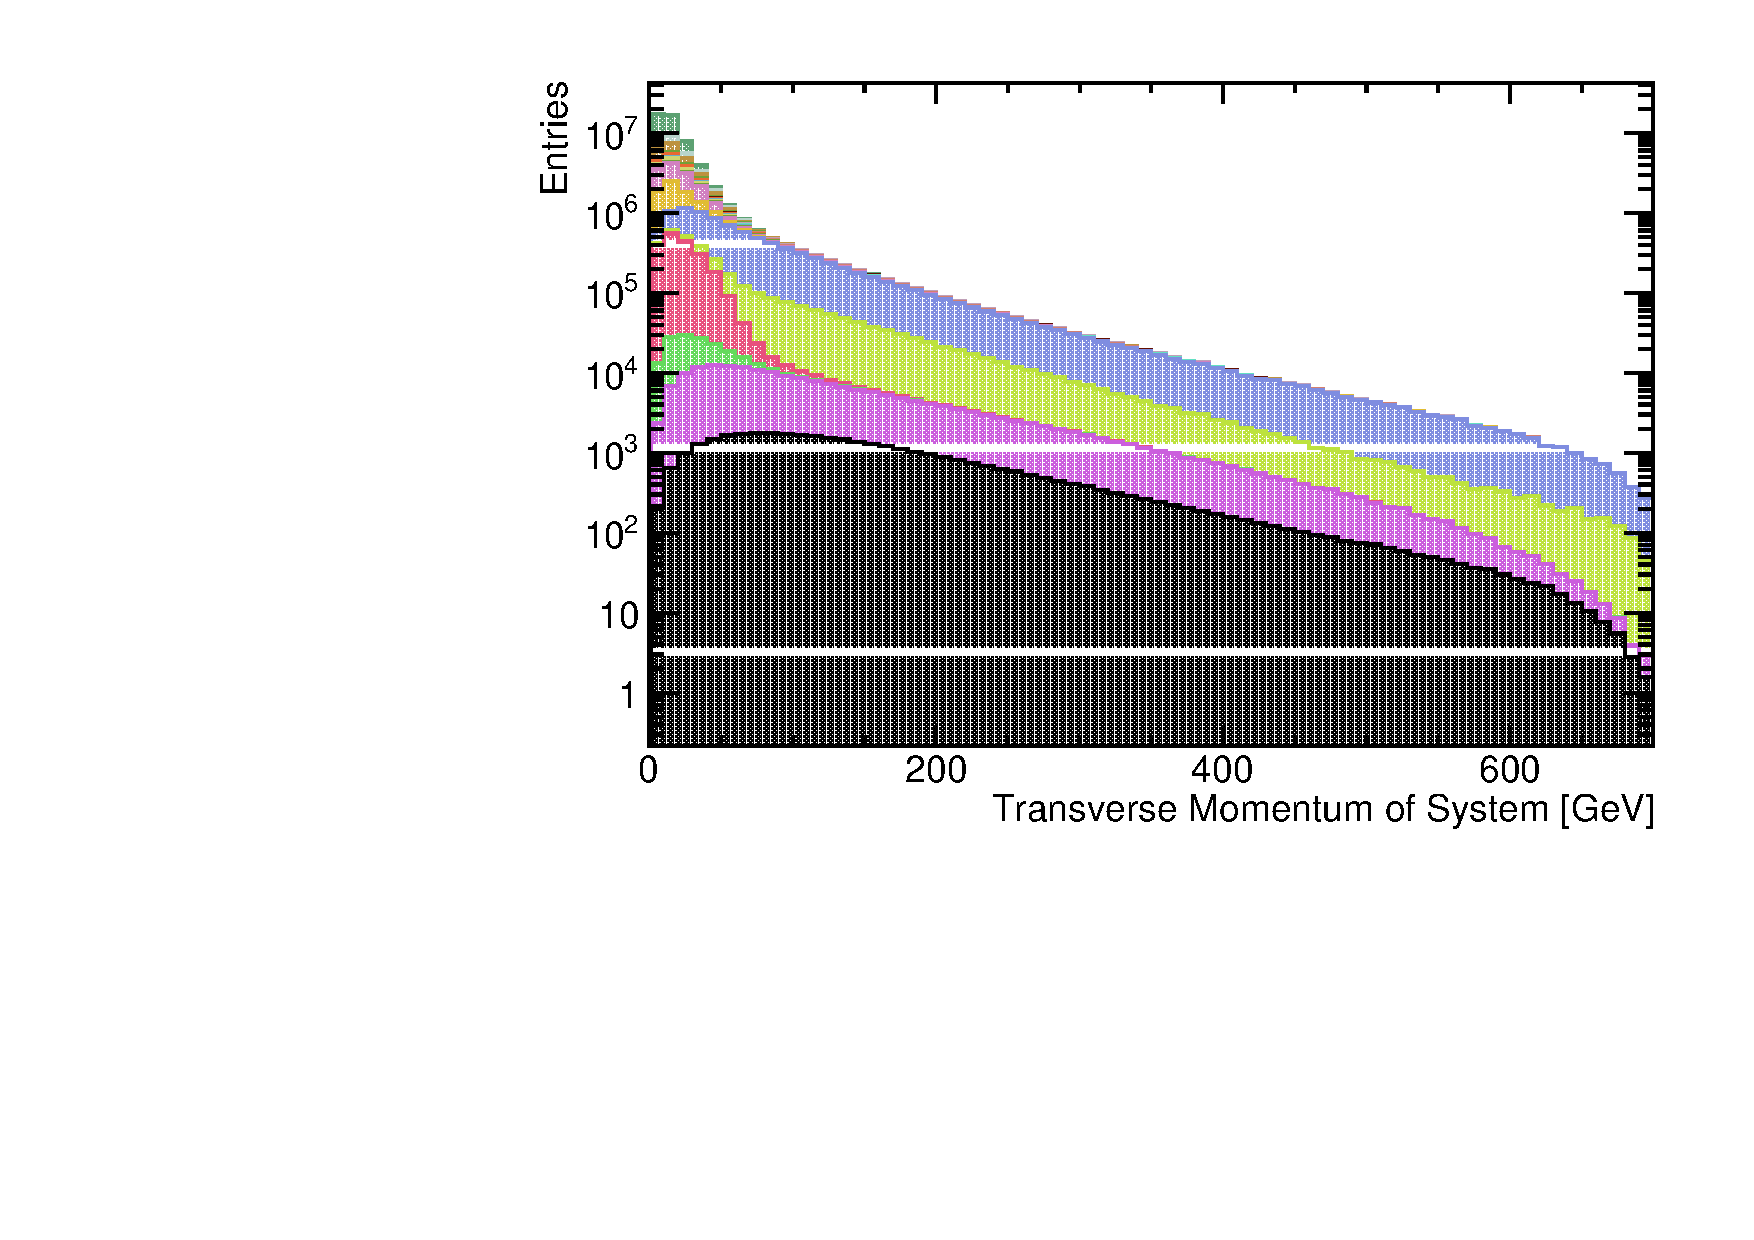
\includegraphics[width=0.75\textwidth]{PhysicsAnalysis/Plots/PreSelection/1400GeV/TransverseMomentum.pdf}
\caption[Transverse momentum at 1.4 TeV.]{The transverse momentum of signal and background events at 1.4 TeV.}
\label{fig:preselection1}
\end{figure}

\begin{figure}
\centering
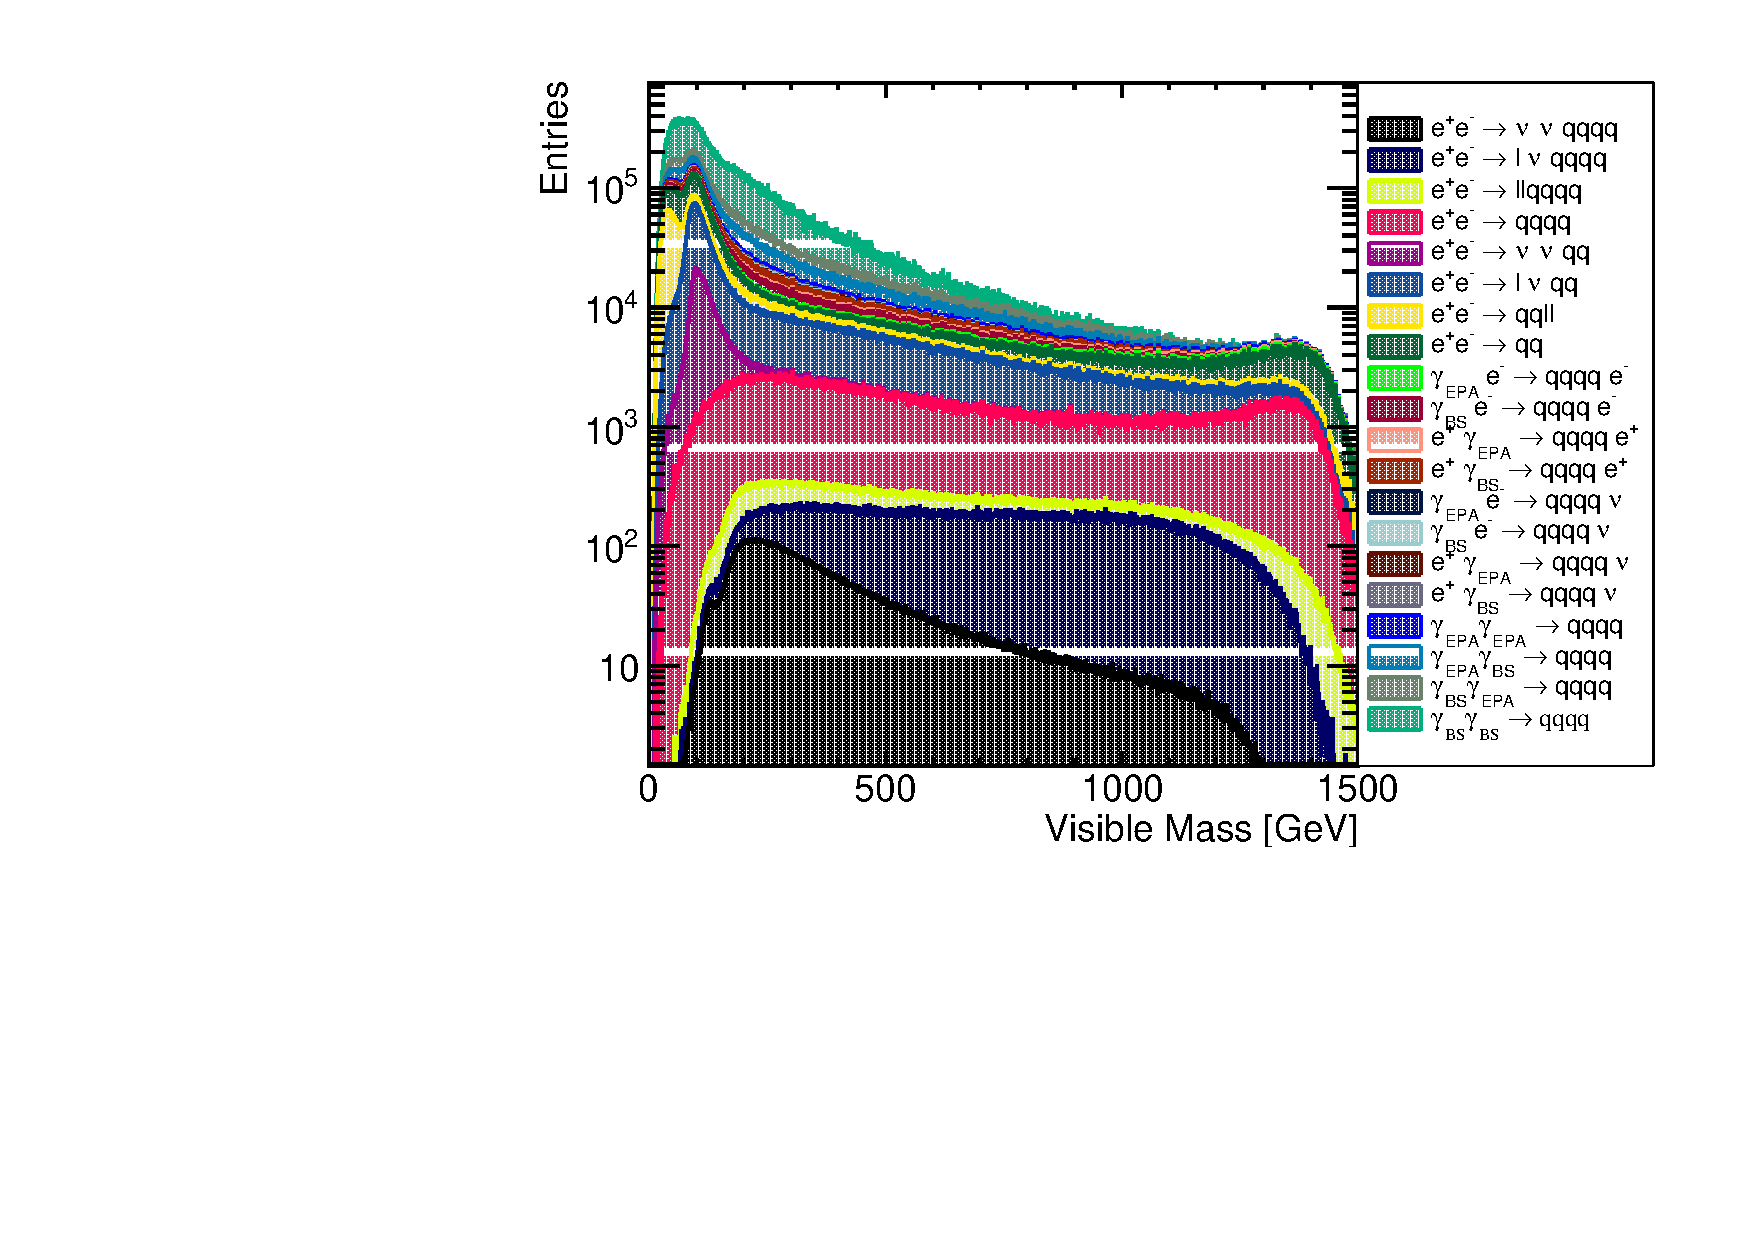
\includegraphics[width=0.75\textwidth]{PhysicsAnalysis/Plots/PreSelection/1400GeV/InvariantMassSystem.pdf}
\caption[Invariant mass of the visible system at 1.4 TeV.]{The invariant mass of the visible system of signal and background events at 1.4 TeV.}
\label{fig:preselection2}
\end{figure}

\begin{figure}
\centering
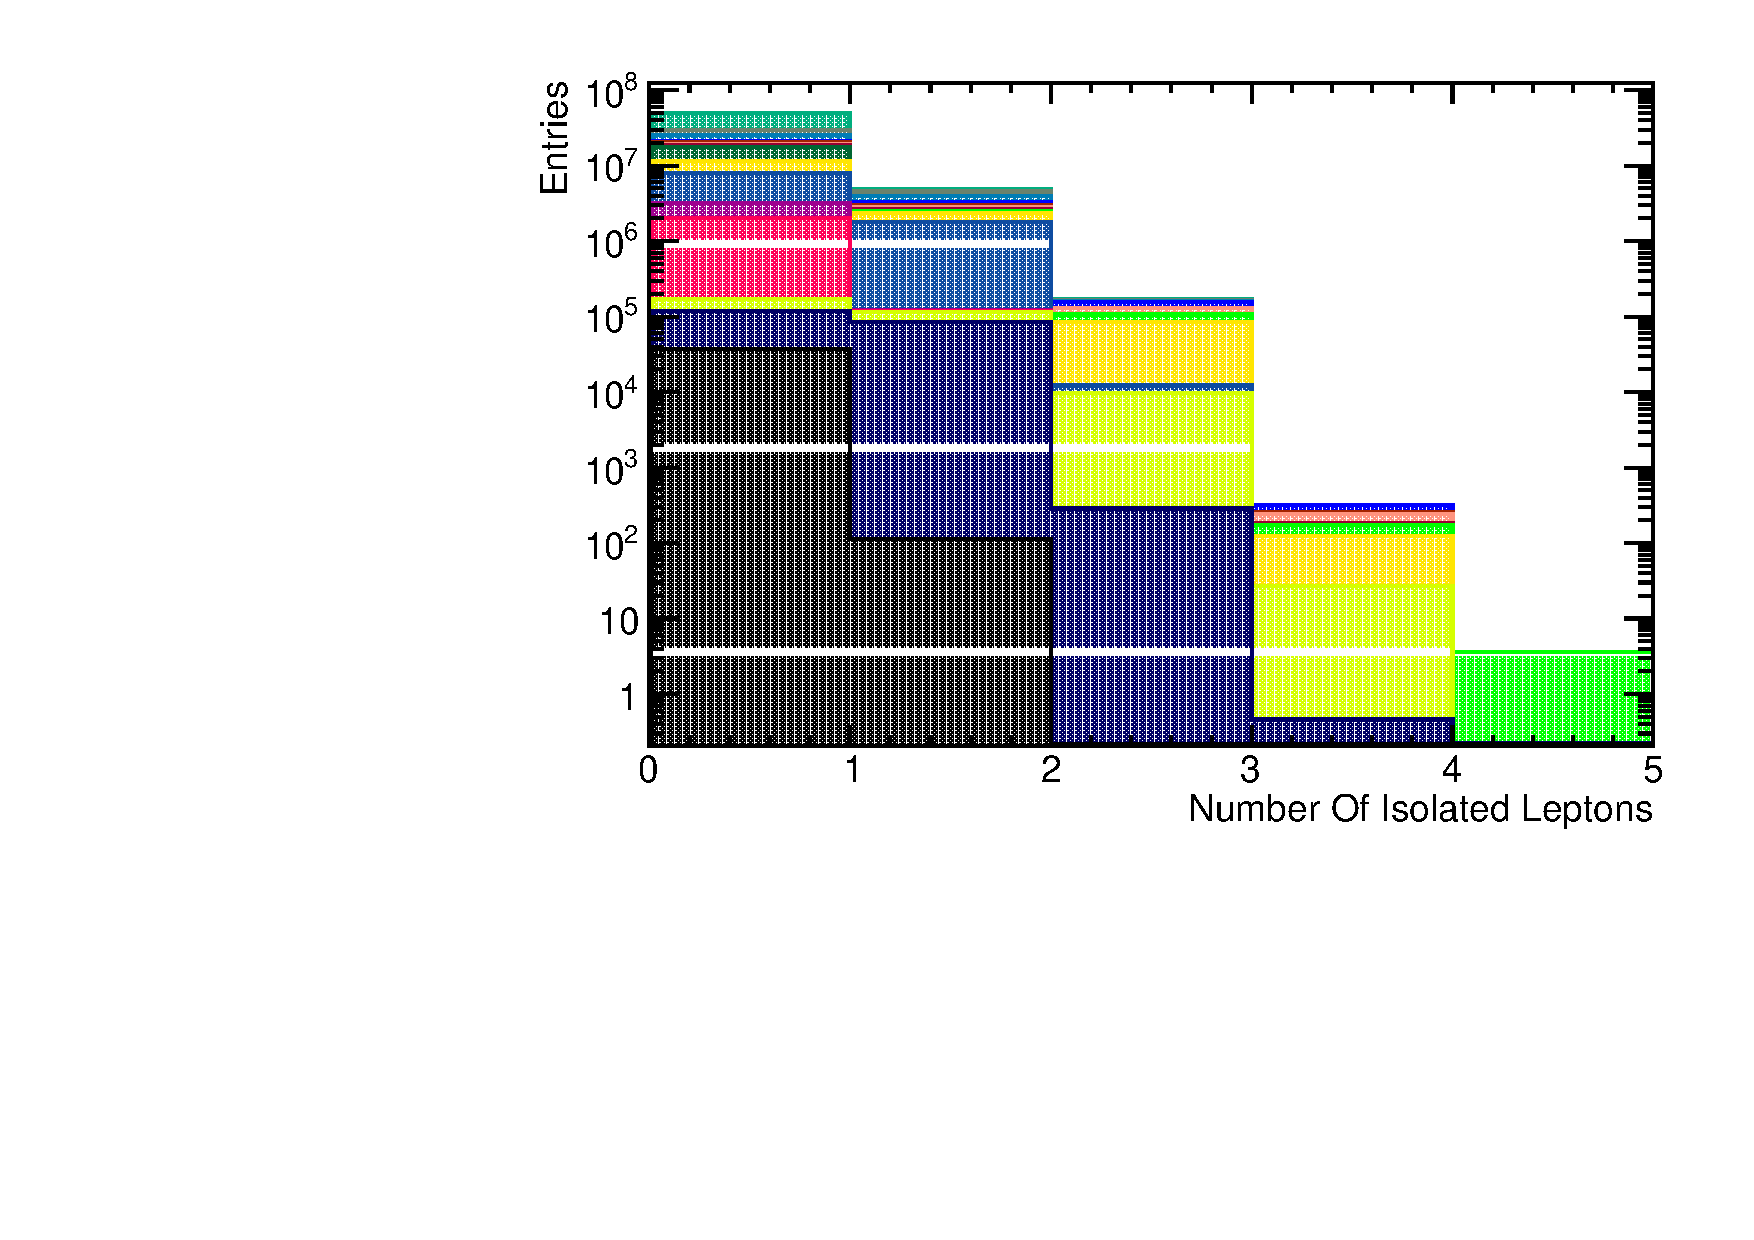
\includegraphics[width=0.75\textwidth]{PhysicsAnalysis/Plots/PreSelection/1400GeV/NumberOfIsolatedLeptons.pdf}
\caption[Number of isolated leptons at 1.4 TeV.]{The number of isolated leptons for signal and background events at 1.4 TeV.}
\label{fig:preselection3}
\end{figure}

\subsection{MVA - 1.4 TeV}
A multivariate analysis is applied to the data set to refine the selection. The following variables were used for training the TMVA selection.

\subsection{Pre Selection - 3 TeV}
\subsection{MVA - 3 TeV}

\section{Fit}

\iffalse
$\text{e}^{+}\text{e}^{-} \rightarrow \nu{\nu}\text{qqqq}$
$\text{e}^{+}\text{e}^{-} \rightarrow \text{l}\nu\text{qqqq}$
$\text{e}^{+}\text{e}^{-} \rightarrow \text{llqqqq}$
$\text{e}^{+}\text{e}^{-} \rightarrow \text{qqqq}$
$\text{e}^{+}\text{e}^{-} \rightarrow \nu{\nu}\text{qq}$
$\text{e}^{+}\text{e}^{-} \rightarrow \text{l}\nu\text{qq}$
$\text{e}^{+}\text{e}^{-} \rightarrow \text{llqq}$
$\text{e}^{+}\text{e}^{-} \rightarrow \text{qq}$
$\gamma_{\text{EPA}}\text{e}^{-} \rightarrow \text{qqqq}\text{e}^{-}$
$\gamma_{\text{BS}}\text{e}^{-} \rightarrow \text{qqqq}\text{e}^{-}$
$\text{e}^{+}\gamma_{\text{EPA}} \rightarrow \text{qqqq}\text{e}^{+}$
$\text{e}^{+}\gamma_{\text{BS}} \rightarrow \text{qqqq}\text{e}^{+}$
$\gamma_{\text{EPA}}\text{e}^{-} \rightarrow \text{qqqq}\nu$
$\gamma_{\text{BS}}\text{e}^{-} \rightarrow \text{qqqq}\nu$
$\text{e}^{+}\gamma_{\text{EPA}} \rightarrow \text{qqqq}\nu$
$\text{e}^{+}\gamma_{\text{BS}} \rightarrow \text{qqqq}\nu$
$\gamma_{\text{EPA}}\gamma_{\text{EPA}} \rightarrow \text{qqqq}$
$\gamma_{\text{EPA}}\gamma_{\text{BS}} \rightarrow \text{qqqq}$
$\gamma_{\text{BS}}\gamma_{\text{EPA}} \rightarrow \text{qqqq}$
$\gamma_{\text{BS}}\gamma_{\text{BS}} \rightarrow \text{qqqq}$
\fi



